
%\documentclass[10pt,letterpaper]{article}
%\usepackage{cogsci}

\documentclass[man,floatsintext]{apa6}

\usepackage[nodoi]{apacite}
\usepackage{graphicx, subcaption}
\usepackage{amsmath}
\usepackage[american]{babel}
\usepackage[section]{placeins}
\usepackage{subcaption}
\usepackage{soul} % for \hl
\usepackage{color}
%\renewcommand\bibliographytypesize{\footnotesize}
\usepackage{pslatex}
% \usepackage{multirow}

\title{Desirable difficulties during the development of active inquiry skills}
\shorttitle{Desirable difficulties in active inquiry}
\author{
 George Kachergis, Marjorie Rhodes, \& Todd Gureckis \\
  \{george.kachergis, marjorie.rhodes, todd.gureckis\}@nyu.edu
}
\affiliation{Department of Psychology, New York University \\
  New York, NY}


\abstract{
This study explores developmental changes in the ability to ask 
informative questions, hypothesizing a link between the ability to 
update beliefs in light of evidence and the ability to ask informative questions. 
Five- to ten-year-old children 
played an iPad game asking them to identify a hidden insect. Learners could either 
ask about individual insects, or make a series of feature queries (e.g., ``Does the 
hidden insect have antenna?'') that could more efficiently narrow the hypothesis 
space. Critically, the task display either helped children integrate evidence 
with the hypothesis space or required them to perform this operation themselves.  Our prediction
was that assisting children with belief updating would help them formulate more informative
queries.  Although this assistance improved some aspects of their active 
inquiry behavior, children required to update their own beliefs asked questions that 
were more context-sensitive and thus informative.  The results show how making a 
task more difficult may actually improve children's active inquiry skills, thus 
illustrating a type of ``desirable difficulty" for reasoning.\\
\textbf{Keywords:} 
question asking, information search, active inquiry, hypothesis testing, scientific 
reasoning}

\begin{document}
\maketitle
\section{Introduction} 

%Figuring out how to efficiently navigate a hypothesis space--
%from learning the diagnostic features to asking the appropriate questions to 
%appropriately updating the space in the face of new evidence--is an essential part of 
%science, and of life, in general. 
%A central part of science--and life, in general--is figuring out how to understand our environment. 
%A variety of conceptual and analytical skills are required in order to detect patterns in 
%environments that initially appear chaotic, and to abstract the general principles that can 
%be used to understand and predict events. A skill of central importance is learning how to ask 
%informative questions to reveal hidden features when they are not immediately obvious.
%In order to discover knowledge, whether in a real science experiment or 
%merely when figuring out a new toy or gadget, children must learn: 1) which 
%observable features are relevant to test, 2) how to intervene on the world in a 
%context-sensitive manner in order to gather additional information about hidden 
%feature values, and 3) how to integrate new evidence to update their hypothesis space.
%
%
%% only keep all the sensemaking framing in the journal paper?? JOURNAL
%The idea of ``sensemaking'' is one useful way to understand the cognitive capacity and process of knowledge discovery \cite{Renner:2011}. Sensemaking, as it is understood in the cognitive and human-
%computer interaction literature, refers to the process of generating meaningful 
%explanations or understandings for possibly incomplete or noisy data patterns in the 
%environment \cite{Russell:1993,Klein:2006a,Klein:2006b}. In contrast to simple 
%pattern recognition or categorization, sensemaking is a highly-volitional process that 
%involves the continual evaluation of new evidence or data, and repeated information 
%gathering. As such, the cognitive processes underlying sensemaking are often 
%conceptualized as a loop where one component process feeds into the next in a 
%repeating sequence, as shown in Figure~\ref{fig:sensemaking_loop}.
%
%\begin{figure}[!h]
%  \centering
%  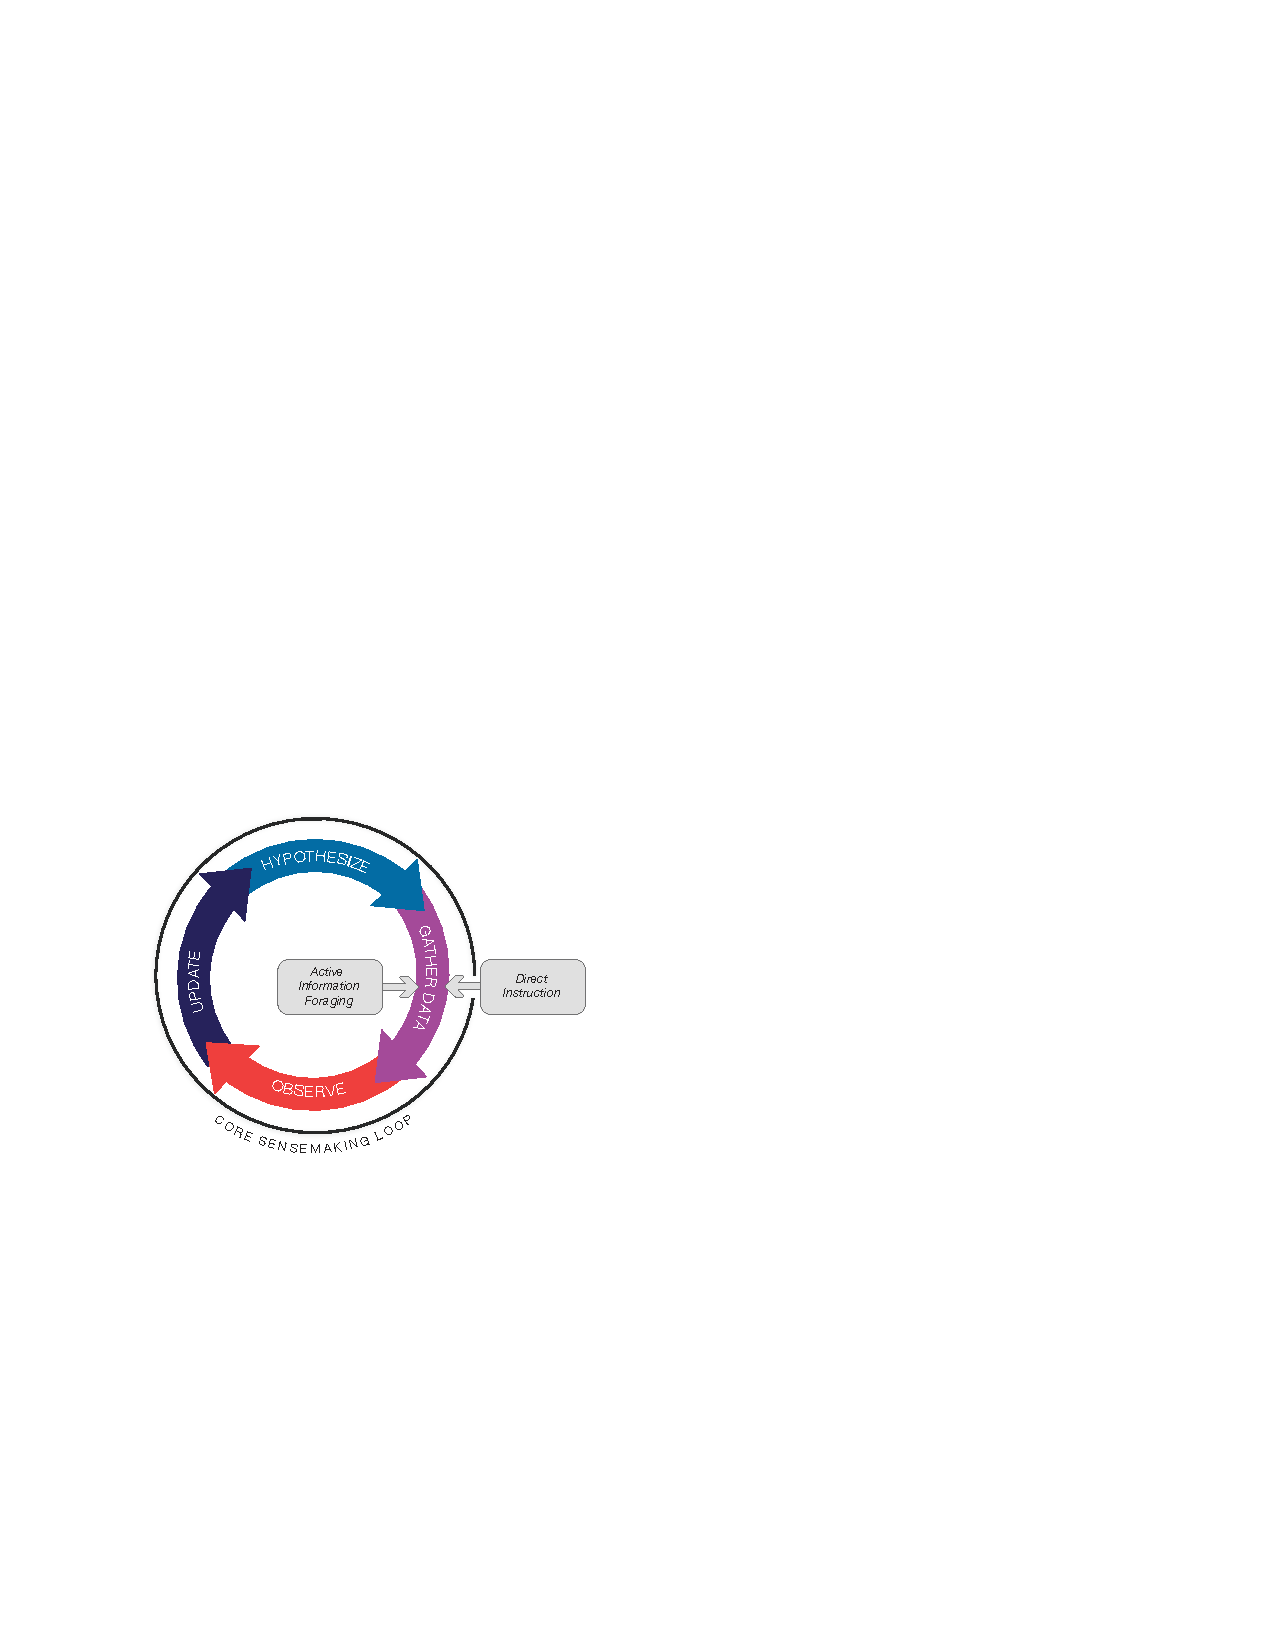
\includegraphics[width=0.45\textwidth]{figures/sensemaking_loop}
%  \caption{The sensemaking loop depicts the successive cognitive process that are 
%engaged when attempting to derive a meaningful understanding of an initially 
%ambiguous situation. The stages of the loop closely mirror the process of scientific 
%reasoning engaged by scientists. However, a similar set of inductive processes are 
%at play in many real-world situations (e.g., working an unfamiliar ATM machine, 
%reading a complex nutrition label).}
%  \label{fig:sensemaking_loop}
%\end{figure} 

%While the sensemaking loop just described is fairly abstract, the goal of the 
%present study is to test and elaborate this theory with the aim of better 
%understanding how to structure formal and informal learning experiences in 
%developmentally appropriate ways. 
% JOURNAL
%This basic sensemaking framework can be instantiated as a computational 
%information processing model \cite{Gureckis:2012,Gureckis:2009,Markant:2012}. 
%The advantage of this formal model is that it allows detailed, testable predictions 
%about behavior. The model-based theory suggests possible bottlenecks that might 
%serve as developmental limitations on learning. For example, young learners may be 
%able to correctly update their beliefs about a set of hypotheses given a set of data, 
%but have trouble using the remaining hypothesis space to guide future information 
%search. The present study explores the development of the data-gathering and updating 
%stages in children, with the aim of developing a more complete understanding of how 
%learning abilities change across childhood.

%Two-year-olds can ask "What�s that?", but younger children can ask the same question by pointing and saying something like "Wha?", "Tha", or "Eh?". (Max said "Doh?"). 
% Nelson�s (1973) seminal study of 18 children�s first words, she found that most had a word that was used in just this way before they learned 50 words�and six of the children had one among their first ten words.

A skill of central importance during development is learning how to ask informative questions
in order to make sense of the world.  
The roots of these abilities are observable even in the early preschool years. 
For example, in simple causal reasoning tasks, preschool-aged children can 
distinguish confounded from unconfounded evidence to draw causal inferences 
\cite{Gopnik:2001,Kushnir:2005,Kushnir:2007,Schulz:2004}. Preschool-aged 
children also selectively explore confounded evidence in their own exploratory play 
\cite{Cook:2011,Gweon:2008,Schulz:2007}. 
%Thus, preschool-aged children show 
%emerging abilities to gather information strategically, distinguish confounded 
%from unconfounded evidence, and to engage in causal inference from limited samples.
%
Despite these early emerging abilities, many of the cognitive skills required for self-guided, active inquiry seem
to follow protracted developmental trajectories. For example, in tasks designed to assess scientific 
reasoning abilities, children in the older elementary school years (ages 8-10) often 
have difficulty adopting systematic strategies, such as testing the effects of one 
variable at a time or selecting interventions that will lead to determinate evidence 
\cite{Chen:1999}. Although children in the older elementary school years can be 
taught to engage in these strategies via direct instruction \cite{Klahr:2004,Kuhn:2005}, 
it is notable how difficult it is for them to discover and implement them on their own. 

One reason for the difficulties children exhibit in these types of inquiry tasks may be that 
active inquiry depends on the coordination of a variety of 
component cognitive processes~\cite{Bonawitz:2010pb,Coenen:2015nr}.
For example, according to one popular view, active inquiry unfolds as a sequence
of mental steps (see Figure~\ref{fig:sensemaking_loop}).  Learners must generate 
possible hypotheses to explain their environment.  They then must engage in 
decision making to ask questions or gather additional information to decide which of
these hypotheses is most likely.
They then must understand the results of these inquiry behaviors and update their 
beliefs accordingly, and so on.  The various 
stages of this loop closely mirror the process of scientific reasoning engaged by 
scientists~\cite{Russell:1993,Klein:2006a,Klein:2006b}. 
Inefficiencies in any or all of these interrelated processes may serve as developmental limitations.  
For example, young learners may be able to search efficiently for information given a particular 
set of hypotheses but have trouble updating their beliefs correctly given new evidence.
In this sense active inquiry behavior is like a bicycle: when all the elements are properly functioning
and aligned the bike moves forward.  
However, misalignment of even one component can be catastrophic.
% and it is reasonable to expect
%that knowledge gathering in younger children may suffer greatly even if they are only having trouble
%with one stage, such as hypothesis updating.

\begin{figure}[!h]
  \centering
  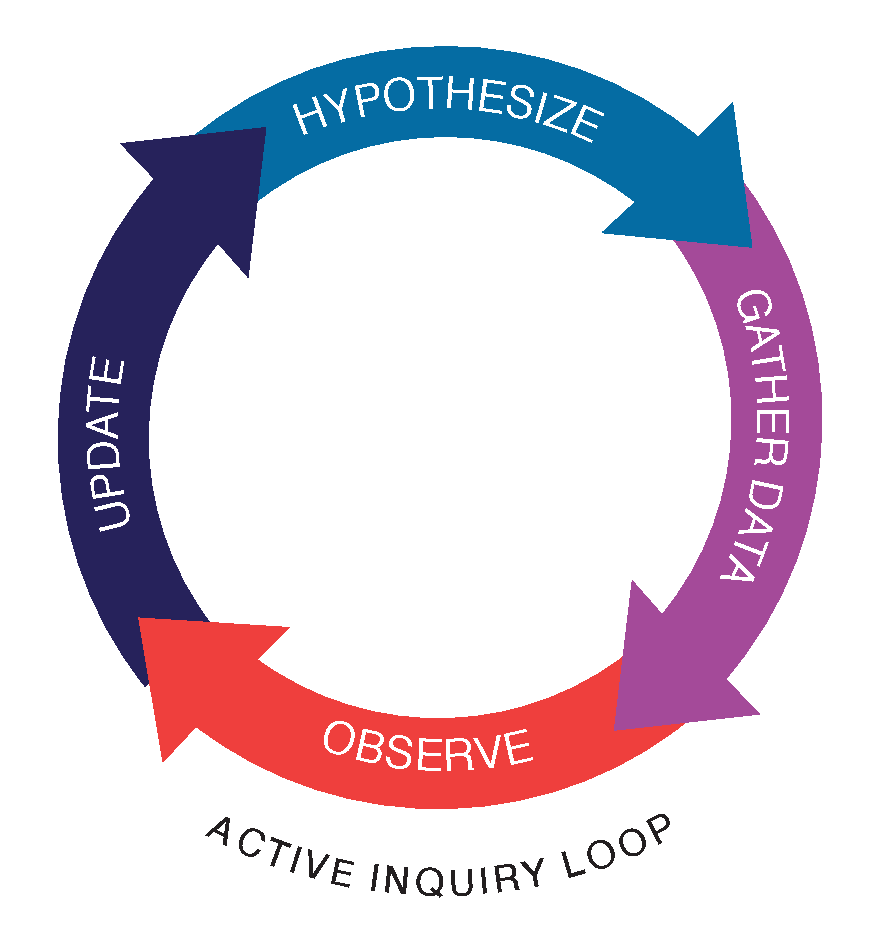
\includegraphics[width=0.40\textwidth]{figures/sensemakingloop}
  \caption{The active sensemaking loop depicts the successive cognitive process that are 
engaged when attempting to derive a meaningful understanding of an initially 
ambiguous situation. The stages of the loop closely mirror the process of scientific 
reasoning engaged by scientists. However, a similar set of inductive processes are 
at play in many real-world situations (e.g., working an unfamiliar ATM machine, 
reading a complex nutrition label).  Aspects of the loop are directly related to 
Bayesian models of learning and information gathering (Bonawitz \& Griffiths, 2010; Gureckis \& Markant, 2009).}
  \label{fig:sensemaking_loop}
\end{figure} 
\nocite{Bonawitz:2010pb,Gureckis:2009}


% this par is repeats earlier sensemaking description:
%However, a similar set of 
%inductive processes are at play in many real-world situations (e.g., working an 
%unfamiliar ATM machine, reading a complex nutrition label).

%update their beliefs about a set of hypotheses given a set of data, but have trouble 
%using the remaining hypothesis space to guide future information search. 

%The present study offers a fine-grained analysis of how question asking develops 
%between the rudimentary abilities of kindergartners and the more sophisticated 
%scientific reasoning skills of older children. 

Understanding the integrated nature of these cognitive processes is important
not just for our scientific understanding of the development of the human mind,
but also because of broader educational implications.  For example, many educational philosophies
emphasize relatively unstructured, self-guided learning environments~\cite{Bruner:1961vn,Kolb:1984mi,Steffe:1995qf}.  
Understanding limitations in children's active inquiry abilities and how each component of such abilities evolves
across age can be used to design more effective learning environments for children of various ages.
For example, evidence that younger children benefit from assistance in updating their beliefs in response to new evidence
would suggest that learning environments for younger children need to provide support for this component of their learning.

%The present study attempts to provide a fine-grained analysis of what develops between the 
%rudimentary abilities of preschool-age children and the more sophisticated scientific reasoning 
%skills of older children.  
%In particular, we join with recent work which attempts to decompose the 
%component processes involved in active inquiry \cite<e.g.,>{Bonawitz:2010pb,Markant:2014}. 
The present study attempts to decompose the 
component processes involved in active inquiry, specifically focusing on the role of 
belief updating.
We tasked five- to ten-year old children to identify a hidden insect in
a simple iPad variant of the classic ``Guess Who?" game. 
Children sequentially asked questions to try to identify the hidden target and received truthful answers.
Based on prior work reviewed below~\cite<e.g.,>{Mosher:1966}, we expected younger children to have difficulty formulating informative queries
and thus sought to explore what types of automated assistance might aid children's reasoning strategies.
Specifically, we manipulated whether the computer program 
helped children to use the new evidence that resulted from their queries to narrow down the
hypothesis space, or whether children had to use the new evidence to reconcile the revealed evidence and the hypothesis space
on their own.  Our expectation was 
that helping children to update their beliefs accurately following the receipt of new information would free up 
cognitive resources and lead to higher quality question-asking. 
Interestingly, our results opposed this initial hypothesis in that elements which 
ostensibly made our task more difficult actually improved the quality of children's inquiry behavior and
suggest an important nuance of the information processing model summarized in Figure~\ref{fig:sensemaking_loop}.
%(was ``important refinement'') ..want to suggest some implication of our finding

%One broader implication of this work is to understand the types of assistive elements which
%support children's reasoning skills, particularly in a museum science setting.
%This study explores the development of the data-gathering and updating stages in children, with 
%the aim of developing a more complete understanding of the learning abilities of young children. First, we review the findings and methods of previous developmental studies of question-asking.
%This work was conducted within the context of an informal science museum
%environment, and we conclude with implications of our findings for the design of
%self-guided educational displays 

%hypothesis was that, although the components of the sensemaking model described above are sequential, they
%likely rely on a common pool of cognitive and attentional resources and are thus not completely
%independent.  In light of this, our 

\subsection{Developmental change in the ability to ask revealing questions}

Active inquiry fundamentally depends on the ability of learners to construct actions or queries
which gain information (e.g., asking a question of a knowledgeable adult).
A now classic way to study this behavior is through experimental tasks based on the 20-questions or 
`Guess Who?" game.
In the game, the asker (participant) tries to determine a hidden object known
only to the the answerer (experimenter) by asking a series of yes-or-no questions.
\citeA{Mosher:1966} identified two broad question types commonly used in the game: \emph{hypothesis-scanning} 
questions test a single hypothesis or specific instance (e.g., ``Is it a monkey?''), whereas 
\emph{constraint-seeking} questions attempt to constrain the hypothesis space faster by 
querying features that are present or absent in multiple objects (e.g., ``Is it soft?''), 
but that do not directly identify the answer except by virtue of elimination. 

A classic finding in this literature is that younger children (e.g., aged 6) tend to ask more hypothesis-scanning questions, while older children (e.g., aged 11) use more constraint-seeking  questions, and also 
tend to find the answer after fewer questions \cite{Mosher:1966}. 
One explanation is that only older children have developed the ability to focus on the 
high-level features that group the hypotheses, whereas younger children focus on individual stimuli.
Consistent with this viewpoint, manipulations that help children focus on these higher-level features, such as cuing them with basic level category labels instead of exemplar names 
\cite{Ruggeri:2015front}, increase the likelihood that young children will generate constraint-seeking questions (see also Herwig, 1982).
Further, although young children are often relatively less likely than older children to ask constraint-seeking questions, even younger children (ages 7-9) are 
more likely to do so when such questions are particularly informative, such as when the hypothesis space is large and there are several equally probable solutions remaining \cite{Ruggeri:2014,Ruggeri:2015}.  Such results are somewhat consistent with the model described above because having the right set of hypotheses, or at least
the right types of category information, in mind seems to drive more effective information search.
\nocite{Herwig:1982}
% (e.g., Ruggeri \& Lombrozo, 2015; 2015).

The behavioral distinction between constraint-seeking and hypothesis-scanning questions can also be studied 
from the normative perspective of information gain, mathematically defined below. 
Intuitively, the most informative question is one that will eliminate half of the remaining hypotheses. 
A question with low expected information gain (EIG) would concern a feature of only one item (e.g., a hypothesis-scanning question) in a large hypothesis space: there is a high probability of eliminating only that single hypothesis (barely reducing the space)--although there is a small chance of eliminating all others. 
However, it is important to note the context-sensitivity of EIG: as it is calculated with respect to the remaining hypothesis space, the relative value of constraint-seeking questions may vary, depending on 1) the presence of features that nearly bisect the space, and 2) the number of hypotheses remaining. In the extreme, with only two hypotheses remaining, there is no informational difference in making a maximally informative constraint-seeking question or simply scanning one of the hypotheses. 
EIG has often been proposed as a model of how children might evaluate the quality of possible queries.  
For example, \citeA{Nelson:2014} found that 8-10 year-old children can search a familiar structured domain 
(people with varying gender, hair color, etc.) fairly efficiently, tending to ask about frequent real-world features 
that roughly bisected the search space (e.g., gender first). 
 Likewise, \citeA{RuggeriXu:2015} found that children's patterns of search decisions were well-explained in terms of EIG.
%\hl{Maybe we can say a little more about EIG here. the context-sensitive analysis of question quality is really important.  
%I think we want to prime the reader for "moving beyond" analyses of constraint vs. scanning
%and focus on context sensitive information measures.  Keep this comment in mind when approaching
%the rest of the paper because there might be a few places to make adjustments in the way we discuss
%things.  for example some of the longer text on EIG of the next subsection might be more appropriate here
%if we discuss context-sensitivity}

 %\citeA{Ruggeri:2015} studied 7-8 year-olds, 9-11 year-olds, and 17-18 year-olds 
%asking questions to identify the cause of an event in real-world scenarios (e.g., Why 
%is a man late to work?). All age groups in that study used more constraint-seeking 
%questions when hypothesis-scanning was unwise: e.g., when the problem had a 
%large hypothesis space or when not all solutions were equiprobable.

\subsection{Belief updating and active inquiry}

While it is clear there are developmental changes in how children formulate questions, less work has considered 
developmental changes in how children make use of the new evidence that their questions reveal~\cite<but see>{Denison:2013kk}.  
However, there are many reasons to think that these two behaviors might be deeply intwined.
The active inquiry loop in Figure~\ref{fig:sensemaking_loop} suggests one obvious interaction because if
questions or information gathering actions are made on the basis of current beliefs, and those beliefs
are wrong, then inquiry will be less effective~\cite<c.f., research on the hot stove effect,>{Denrell:2001mw,Rich:2015qo}.  
%There are certainly many examples where scientific progress has been derailed by incorrect interpretation of evidence.
%\nocite{Needham:1745ff}


\nocite{Coenen:2015nr}
Coenen and Gureckis (2015) describe a more fundamental reason for why belief updating and information
search might be related.  In particular, they focus on a popular computational model of active inquiry
called Expected Information Gain (EIG).  This model has been widely used in both the adult and developmental
literature to understand how people decide between different queries~\cite{Oaksford:1994tw,Steyvers:2003ee,Coenen:2014qr,Nelson:2005ph,Gureckis:2009,Markant:2012fk,Nelson:2014,RuggeriXu:2015}, and will be used as a normative benchmark for question quality in the present study.
Intuitively, EIG evaluates the quality of a question by considering how much is expected to be learned from
each possible answer to that question.  For example, in the 20-questions game a child might ask ``Does your
character have a hat?"  or ``Is your character a male?"  To decide between these two queries
EIG considers each possible answer (``yes" or ``no" for both) and how much each answer would alter
the learner's current beliefs given the question.  If all the remaining characters in the game are wearing hats then the
answerer would never respond ``no" to the hat question, but answering ``yes" does not normatively alter the learner's
beliefs.  In contrast, if roughly half the remaining characters were male, then either answer (and therefore the average) to the second
question would strongly shift what the learner knows about the true character.  On this basis the more valuable
question according to EIG would be ``Is your character male?"  In this model, belief 
updating is fundamental to judging the information quality of a possible query: it is only by imagining how one's 
beliefs would change given different answers that a question derives meaning and value.
On the basis of this observation, Coenen and Gureckis (2015) reported a study aiming to relate individual
differences in belief updating during a causal reasoning task to patterns of information seeking behaviors.  
Subjects that showed clear evidence of biased belief updating (e.g., incorrectly interpreting ambiguous 
evidence as unambiguous) also showed biased patterns of information gathering in a causal intervention learning task.  
This study highlights the strongly interactive nature of belief-updating and information seeking behaviors.

Interestingly, past work on the development of question asking abilities in children has tended not 
to emphasize belief updating as a dependent measure, or precluded studying updating beliefs by the design of
the study.  For example, 
\citeA{Herwig:1982} presented children with a series of two-alternative forced choice decisions between 
hypothesis-scanning or constraint-seeking question but did not actually give feedback (and therefore
could not detect errors in belief updating).
In the 20-questions task of \citeA{Nelson:2014}, 8- to 10-year-olds were asked to identify which of 18 people was the hidden target, and played the game to completion several times for different targets. Children eliminated
hypotheses (flipping over cards) based on acquired evidence, but were given help by the experimenter if needed, which presumably means they were not allowed to make errors. 
%%% TODD: sounds weird if it was unclear from the procedure can we attack whoever this is for this?  
%%%I think not but it is sloppy on their part. otherwise just say they weren't allowed to make errors. 
% G: quote from Nelson:2014: 
% "The face cards eliminated through a question were turned over by the child, if needed with help from the experimenter." 
% I assume 'if needed' means if they made a mistake, thus 'presumably' seemed appropriate
 In \citeA{Ruggeri:2014}, the experimenters did not explicitly represent the hypothesis space for participants
in Experiment 1's causal reasoning task (e.g., ``Why was a man late to work yesterday?''), and when ten 
explicit reasons for being late were given in Experiment 2, they remained in view.  That is to say, the process 
of hypothesis updating was not scrutinized in these prior studies.

%Might children be sensitive to this difficulty, and thus seek to avoid errors by using easily-interpretable hypothesis scanning? Might an intervention that aids with hypothesis updating encourage the use of constraint-seeking questions? 
%In this study, we explore how to alter the relative utilization of constraint-seeking
%or hypothesis-scanning via.... display element, helping with updating.  Also we look at developmental changes.

In the present study, we hypothesize that biases in the
way children search for information (e.g., by favoring hypothesis scanning questions over
constraint seeking questions) may stem from difficulties in coordinating the belief updating
and search process.  There are a variety of specific reasons for this prediction.  First, 
although the components of the sensemaking model described in Figure~\ref{fig:sensemaking_loop}
above are sequential, they likely rely on a common pool of cognitive and attentional resources and 
are thus not completely independent.  In this case the cognitive load from planning questions,
or from updating beliefs, may impair performance on either task.
Second, hypothesis scanning questions might be easier for young children is that they produce 
evidence that applies to a single hypothesis.  If instead children ask constraint-seeking questions, 
they must eliminate from the hypothesis space any possibilities that are ruled out by the new information. 
This process could be cognitively taxing, and also prone to errors. Thus, although constraint-seeking 
questions are often more informative in theory, they might not always be so to young children, particularly 
if children have difficulty using the obtained information to update their representation of the hypothesis 
space accurately. 

To test this hypothesis, in the present study we manipulated whether children received assistance in 
integrating evidence with the hypothesis space or had to undertake this process on their own.  Our
expectation was that aiding children in coordinating evidence and beliefs would enable more sophisticated, and informative,
inquiry behavior.  To evaluate this prediction we evaluated the quality of children's question asking ability
against an objective standard of informativeness given by the EIG model described in more detailed below.
 We additionally analyze our data specifically in terms of constraint-seeking and hypothesis-scanning questions.  
Our central prediction was that assistance in belief updating should increase the relative EIG of children's questions
and the relative utilization of constraint-seeking questions.
Given that older children (8-10 years) have previously been found to use more constraint-seeking questions than younger children (5-7 years), we tested across these two age groups, expecting that younger children
would benefit more from the assistance in hypothesis updating than would older children, and that the manipulation may increase the younger children's use of constraint-seeking questions.

%Together this work is consistent with the view that active inquiry behaviors are deeply linked
%to component cognitive processes such the representation of the task or
%the structure of the hypothesis space. 

%The experimental framework used here is a variant of the ``20 questions'' game, in 
%which the asker (participant) tries to ascertain what object the answerer 
%(experimenter) is thinking of (e.g., ``What have I got in my pocket?'') by choosing 
%and asking a minimal series of yes-or-no questions. Variants used in experiments 
%often present a finite set of familiar kinds of objects, such as animals \cite{Ruggeri:2015front} 
%or people \cite{Nelson:2014}, from which the to-be-discovered answer is 
%randomly selected, and some even provide lists of acceptable questions for askers 
%to choose from. Investigating children aged 6-11 years, 

%However, these studies all used hypothesis spaces that were likely familiar to 
%participants to some extent---and likely to a larger extent for older participants. 
%In contrast, the present study introduces a novel, hierarchically-structured 
%hypothesis space in which the concrete features are randomly assigned. 

% The present study differs from that of \citeA{Ruggeri:2015} in several ways, among them being 
%that the present task: 1) is not a causal inference task, 2) introduces a novel 
%hypothesis space with features' informativeness being randomly assigned, and 3) 
%presents the available strategies (i.e., hypothesis-scanning and constraint-seeking 
%queries) explicitly as side-by-side buttons.
%
%In this study, children (ages 5-10) play multiple rounds of a self-guided 20-questions 
%style iPad game with a structured but novel hypothesis space. 

%We focus here on belief updating.  That this can be a challenge for children to coordinate along with other processes in
%the task (i.e., asking questions).  In addition many theories of active
%information seeking (e.g., information gain) include within the valuation of a
%possible query a belief update step (Coenen \& Gureckis, 2015).  As a result
%one might expect tasks which aid people in performing belief updating might
%also improve their active information seeking.
%
%Todd: In our experiment children attempted to play a version of the Guess
%Who? game.  On each trial children could choose to click a button to obtain
%information about a hidden insect.  There were different types of buttons
%available (exemplars which just allowed children to ask if one specific insect
%was the hidden one) or features (which allowed children to ask if a specific
%property applied to the hidden insect).  These two query button types roughly match
%the distinction in Mosher and Hornsby (1966) concerning hypothesis-scanning
%and constraint-seeking questions.  Our primary manipulation was
%to either help children with the updating step by automatically removing
%from the set any insect which is inconsistent with evidence encountered so far.
%Our primary dependent measure what the sequence and type of button
%presses the children made as they learned to identify the insect.
%\vspace{-.1cm}
\section{Experiment}
%\vspace{-.2cm}
The purpose of the experiment is to investigate how children utilize hypothesis-
scanning and constraint-seeking questions when trying to discover a hidden object.
To that end we created 
a tablet-based game based on the popular ``Guess 
Who?'' paradigm.   To increase translational impacts of the project, it was
conducted in the context of a children's science museum and the materials and 
design of the study were selected to integrate with museum content.
Our hope was that insights from the study might be used to help museum curators
design more effective educational exhibits that target children of different ages.
%\hl{Needs to mention age group prediction, feature utility information, hypothesis
%scanning and constraint seeking questions, plan for analysis and evidence that
%we would use to suggest assisting with belief updating would help}
%The purpose of the experiment is to investigate how children utilize hypothesis-
%scanning and constraint-seeking questions when trying to discover a hidden feature 
%in a novel environment, and to ask whether evidence-based belief-updating is a 
%bottleneck in the knowledge discovery process. To address these issues, we created 
%a tablet-based game in the ``20-questions'' style (or more specifically, ``Guess 
%Who?''). Formally, this task involves search of a binary decision tree. To accomplish 
%this search optimally, one should search for and query the feature at each step that 
%most nearly bisects the hypothesis space. 
%We will assess how well  participants monitor their own understanding and how they choose to seek additional 
%information until their understanding is complete. Specifically, we ask how children 
%test hypotheses when they can use a mixture of hypothesis-scanning and constraint-seeking 
%questions in a novel feature space: Do they use feature queries and then scan hypotheses? 
%%Do they gradually learn to test more discriminative features? 
%Do they make queries that are context-sensitive (i.e., relevant to the information state 
%they are currently in)? Does manually updating the hypothesis space reveal 
%bottlenecks, or perhaps push learners to find more informative queries?

\subsection{Methods}
%\vspace{-.1cm}
\subsubsection{Participants}

Participants in this experiment were 134 children between the ages of 5 and 10 
years old who were recruited at the American Museum of Natural History's 
Discovery Room. Of the 134 children recruited, we analyze the data from 121 
children (21 5-year-olds, 20 6-year-olds, 22 7-year-olds, 20 8-year-olds, 20 9-year-olds, 
and 18 10-year-olds) who completed 5 or more rounds of the game.
Participants were assigned in counterbalanced order to either 
the automatic-update condition or the manual-update condition (67 per condition).

\subsubsection{Stimuli}

On each round, children were presented with a display containing sixteen insects.  One of the insects was randomly
selected to be target which children attempted to identify by asking questions.  The sixteen insects within a round shared the same body 
shape but were composed of varying varying perceptual features.  In particular, insects were defined by the presence or absence 
of 9 features: green body, orange eyes, antennae, big spots, tiny spots, 
legs, leaves, water droplets, and blue ``fur''. Figure~\ref{fig:example_bugs} shows an example of two of the body shapes used, 
each with all of the binary features present.   Across rounds the body shapes (selected from a pool of 
16 unique body shapes) varied randomly but within a round the body shape was shared between all sixteen items.  The insect task 
was designed to fit thematically with the content of the AMNH Discovery Room activities which emphasize the often subtle differences 
between species of animals (specifically, many interactive exhibits involve insects).


\begin{figure}[h]
  \centering
  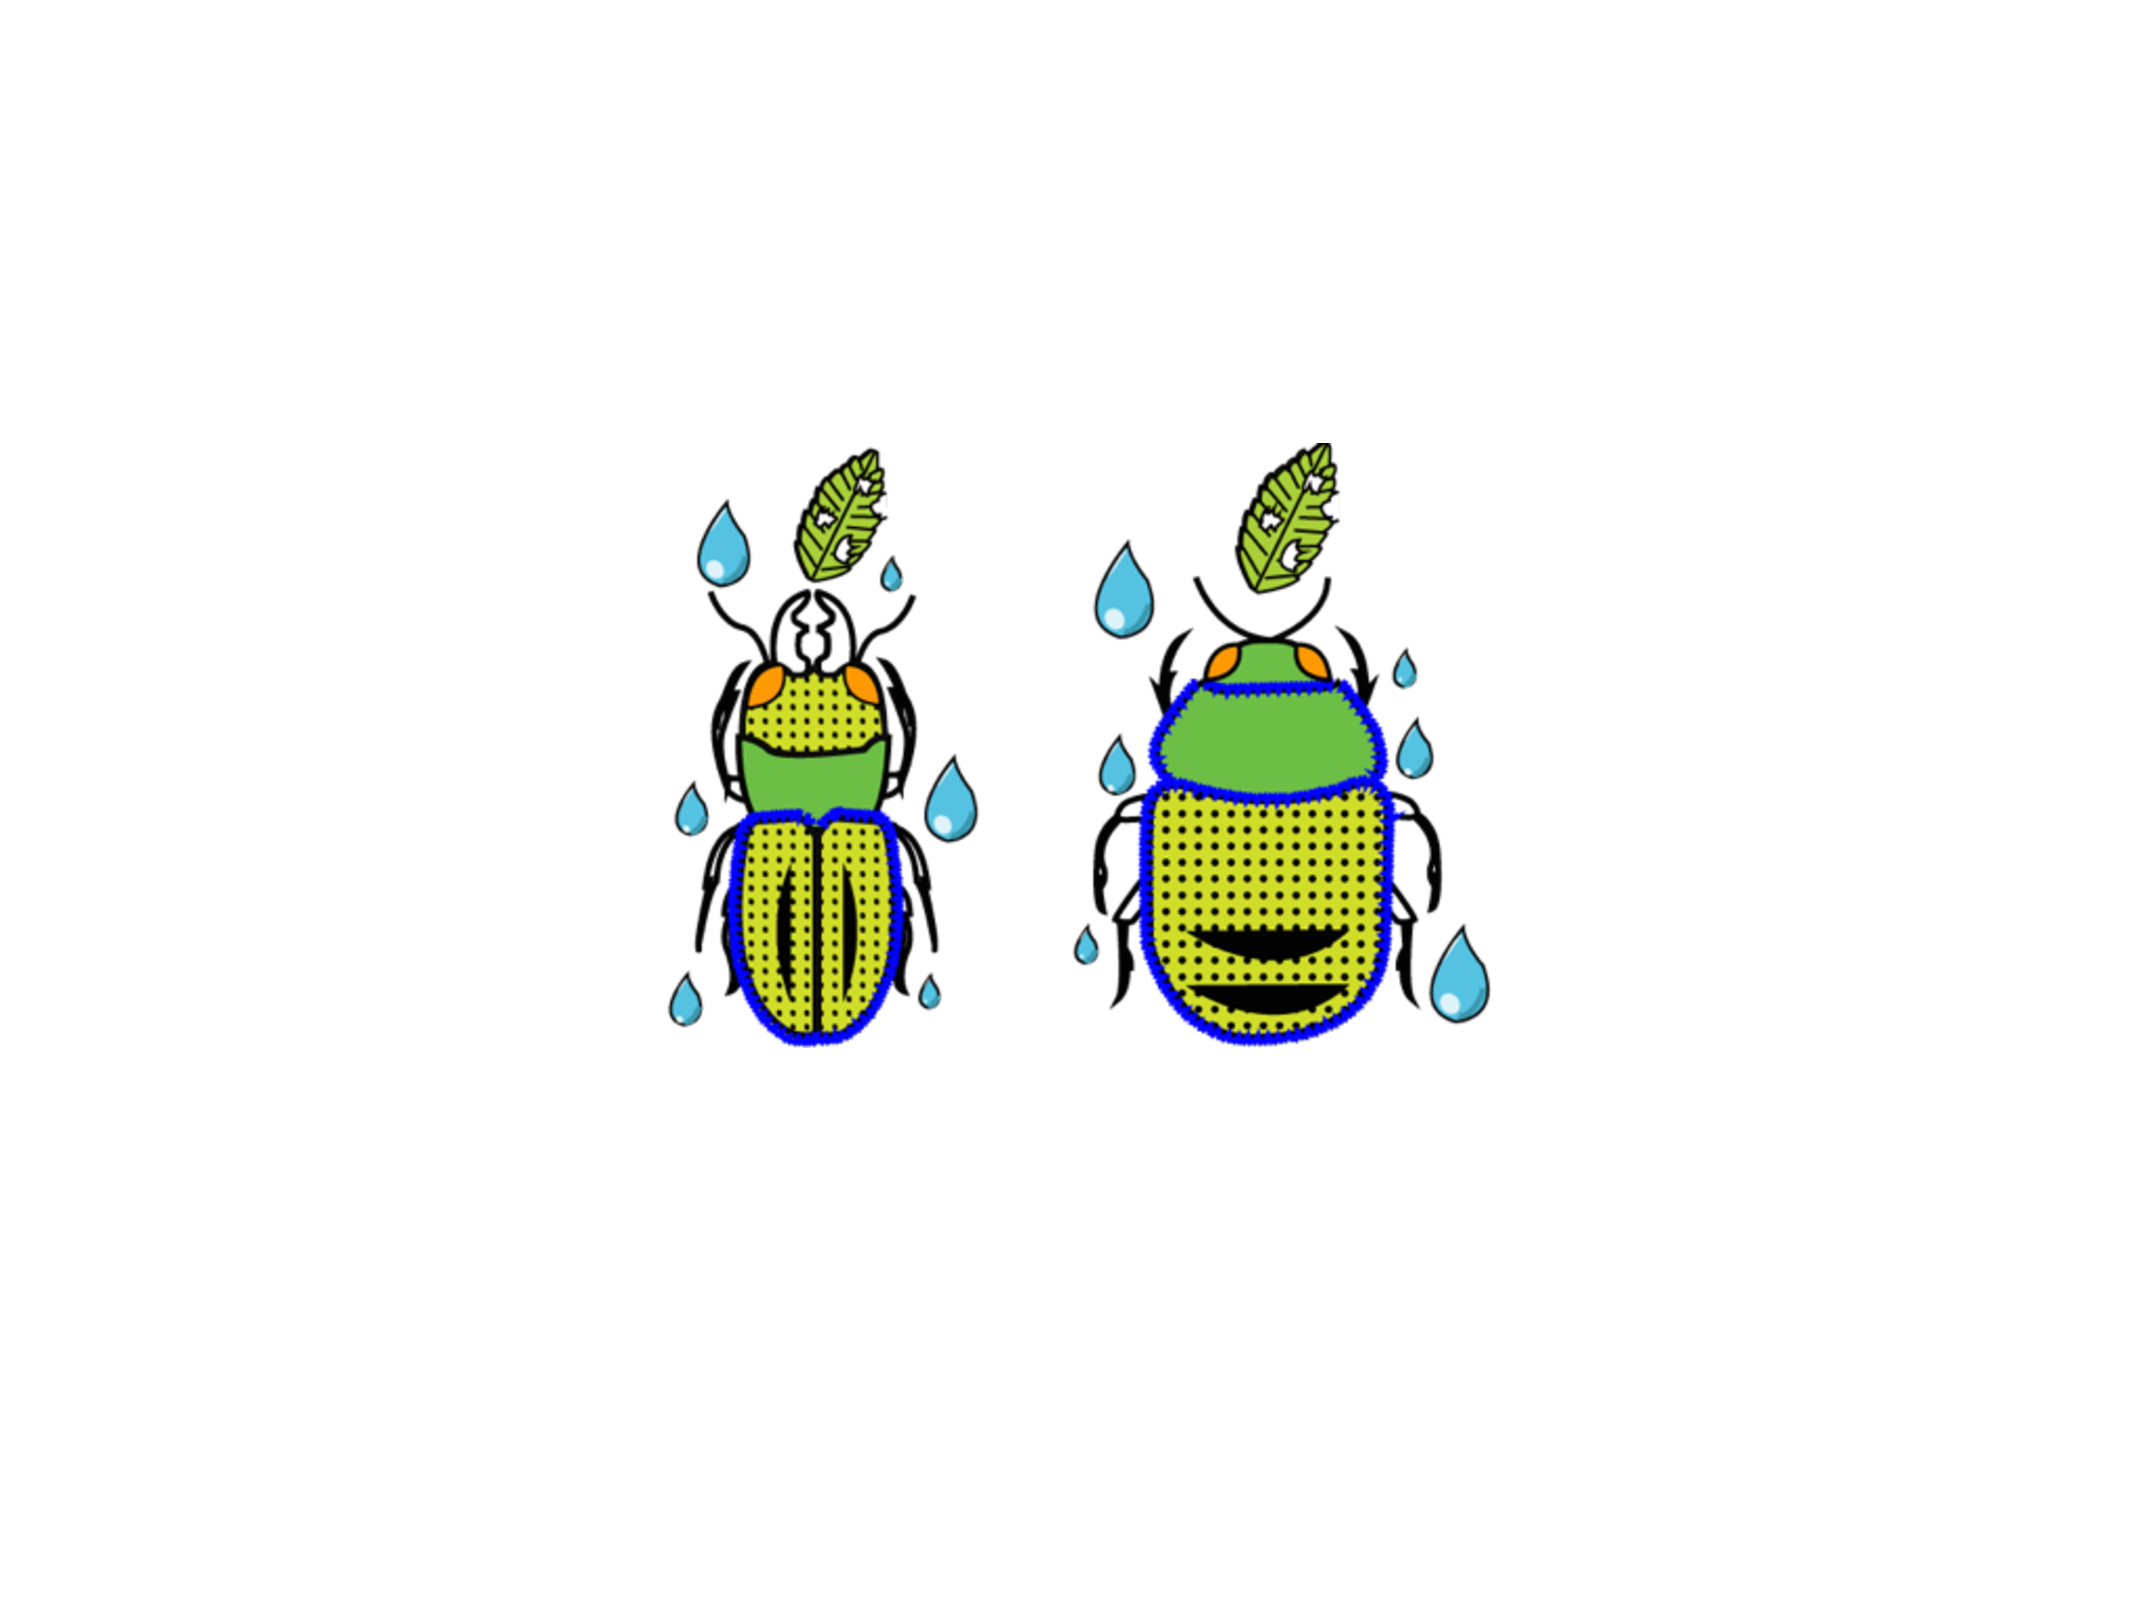
\includegraphics[width=0.4\textwidth]{figures/example_bugs}
  \caption{Examples of two insect body types with all 9 of the binary features present. Each round used one of 16 possible 
body shapes. } % Each insect in a round had a unique combination of features.
  \label{fig:example_bugs}
\end{figure} 

\subsubsection{Design}

Across the sixteen exemplar insects (A-P in Table~\ref{fig:feature_table}), some binary (present or absent) features were more frequent than others (e.g., one was present on eight of the insects), while some were very infrequent (e.g., two were present on only two insects). Table~\ref{fig:feature_table} shows the abstract structure of the feature distribution. The features (F1-F9) in this semi-hierarchy were randomly assigned to the visual features for each 
child (i.e., F1 might be mapped to color (1=green, 0=white) for one child, while F1 is mapped to leaf-eating (1=leaf, 0=no leaf) for another), and then remained consistent across rounds. 
This gave children the possibility to learn the quality of different features across the rounds.
The design of the abstract structure introduced strong differences in the informational utility of each feature (F1-F9).  
For example, given no other information it would be quite informative to ask about feature F1
because it is shared with half of the possible insects.  In contrast, feature
F9 is less informative on the first trial of each round because most of the insects do no have this feature. 

\begin{table}[h]
  \centering
  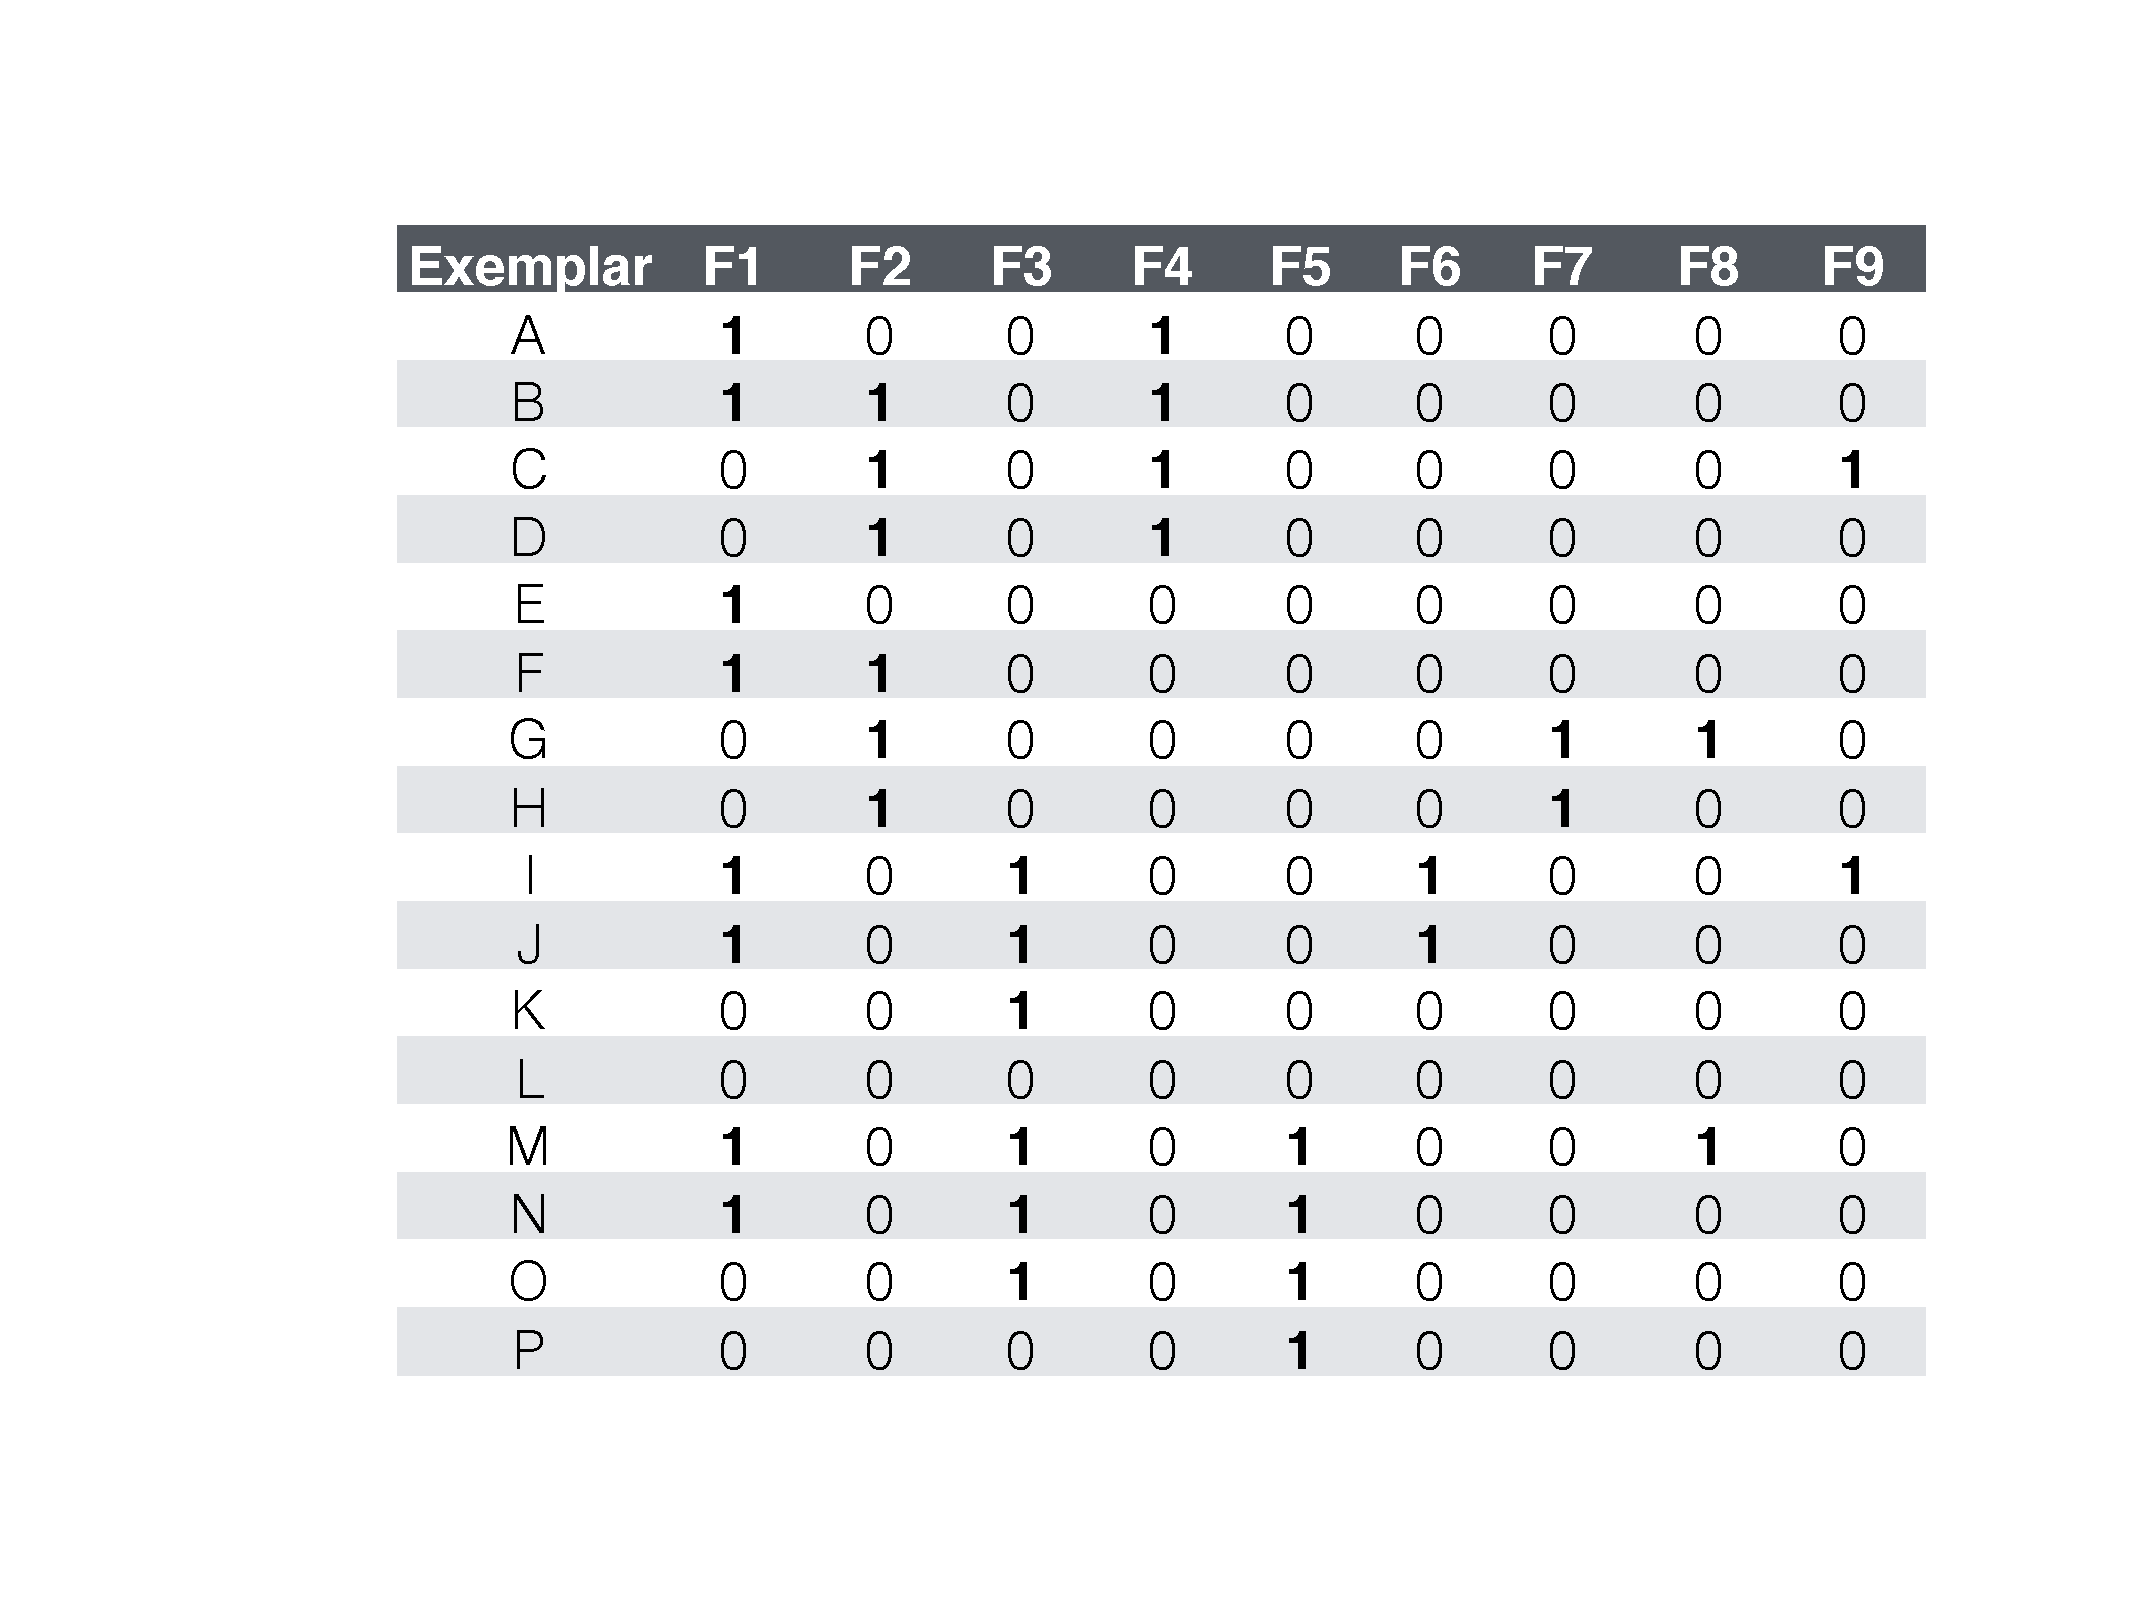
\includegraphics[width=0.55\textwidth]{figures/feature_table}
  \caption{The abstract feature structure of the 16 insects (A-P) used in each round. 
Each child had these abstract features (F1-F9) randomly assigned to the binary (present or absent) visual 
features, but had a consistent assignment used from round to round. }
  \label{fig:feature_table}
\end{table} 

Each of these features was visually represented on a button (see Figure~\ref{fig:task-overview}), available for children to tap with their finger.   An additional feature button depicted a particular body shape was always present but not relevant to the insects on display since they always
shared the same body shape.  A tap on a feature button is effectively a ``constraint-seeking" question. 
Instead of choosing a feature button, children could at any time query an exemplar by tapping it to determine if it was the hidden insect or not. This choice is equivalent to a ``hypothesis-scanning" query.  
The interactive elements of the display varied across conditions.  After making a feature query in the manual-update condition, children must select which insects (i.e., hypotheses) are consistent with the feedback.  In contrast, in the automatic-update condition the hypothesis space automatically updated to be consistent with the feedback received.

\subsubsection{Procedure}

After being trained by an experimenter on a simpler version of the task with unrelated stimuli\footnote{Download 
full task code and instruction scripts: \texttt{https://github.com/kachergis/bugguess}} (a dog searching dog houses) so that they understood how to query exemplars and features, and how 
to eliminate hypotheses, children played 5 or more rounds of an iPad game asking them 
to identify which one of 16 insects was hidden under a cartoon rug (see Figure~\ref{fig:task-overview}). 
The task alternated between the query phase and the elimination phase. In the query phase, 
players could either query an individual insect by tapping one (equivalent 
to asking, ``Is this the hidden bug?''), or choose use a feature query button (e.g., the green button asks 
``Is the hidden bug green?'') to find out whether the hidden insect had a particular feature. 

If a single exemplar was tapped on (i.e., a hypothesis-scanning query), and item was the experimenter-determined
hidden insect, a smiley face appeared and the round was completed.  If the tapped exemplar 
was not the hidden insect, a red ``X'' was shown on top of the tapped insect and the insect becomes 
grayed out (i.e., eliminated). 

After a feature query (i.e., constraint-seeking query), the insect under the rug gives feedback, saying 
``Yes!'' (it has the feature; narrated by the experimenter), or ``No!'' (it does not have 
the feature). This is followed by the elimination phase, during which insect that are 
inconsistent with the feedback are eliminated, and the hypothesis space is thus narrowed. 
The elimination phase varied based on condition.
 In the automatic-update condition, after the feedback from a 
feature query, subjects merely pressed the ``Eliminate'' button and all the no longer relevant insects 
are eliminated (grayed out), and the game returned to the query phase. In the 
manual-update condition, after a subject made a feature query and saw feedback, 
they had to select each insect that was consistent with the feedback for that feature, as 
shown in the top right of Figure~\ref{fig:task-overview}. Insects were selected (denoted by a green box) by 
tapping, and could be deselected by tapping again. Only when children verified they were done 
selecting insects did the experimenter press the ``Eliminate'' button, which eliminated 
any insects that were not selected. 

Before children were allowed to begin, the experimenter explained a random selection of at least three of the feature 
buttons (more if the child asked), and asked children to point to an exemplar exhibiting each of the explained features. 
In the manual-update condition it was possible for mistakes to be made
during the elimination phase, as the software did not aid in updating the hypothesis space. Insects that should have been eliminated but were kept (a `miss') 
continued to be valid options.  Insects that were consistent with the query but wrongly eliminated (a `false alarm') 
were grayed out.   Our analyses below take into account
the role that such errors may have played in the manual-update condition.
In the event that the hidden insect was wrongly eliminated during a manual-update error, 
the round was played out until all of the insect/hypotheses were grayed out. The experimenter would then indicate 
that the insect must have been mistakenly eliminated (but not at what point), and would end the round by 
clicking the grayed-out exemplars until the hidden one was found. These final clicks (beyond when all 
hypotheses were eliminated) were not included in the analysis.  

At the beginning of each round, the experimenter would say, ``Let's try to find which insect is hiding pretty 
quickly, so we can do more!'' Thus, the task mostly relied on intrinsic motivation to solve the puzzle quickly, 
providing no direct cost incentive to be efficient. This was chosen primarily due to the difficulty of rewarding
children in the museum.  Children were welcome to complete more than five rounds, 
if they desired to: after the fifth and each successive round, they were asked, ``Do you want to play again?''

\begin{figure}[!h]
  \centering
  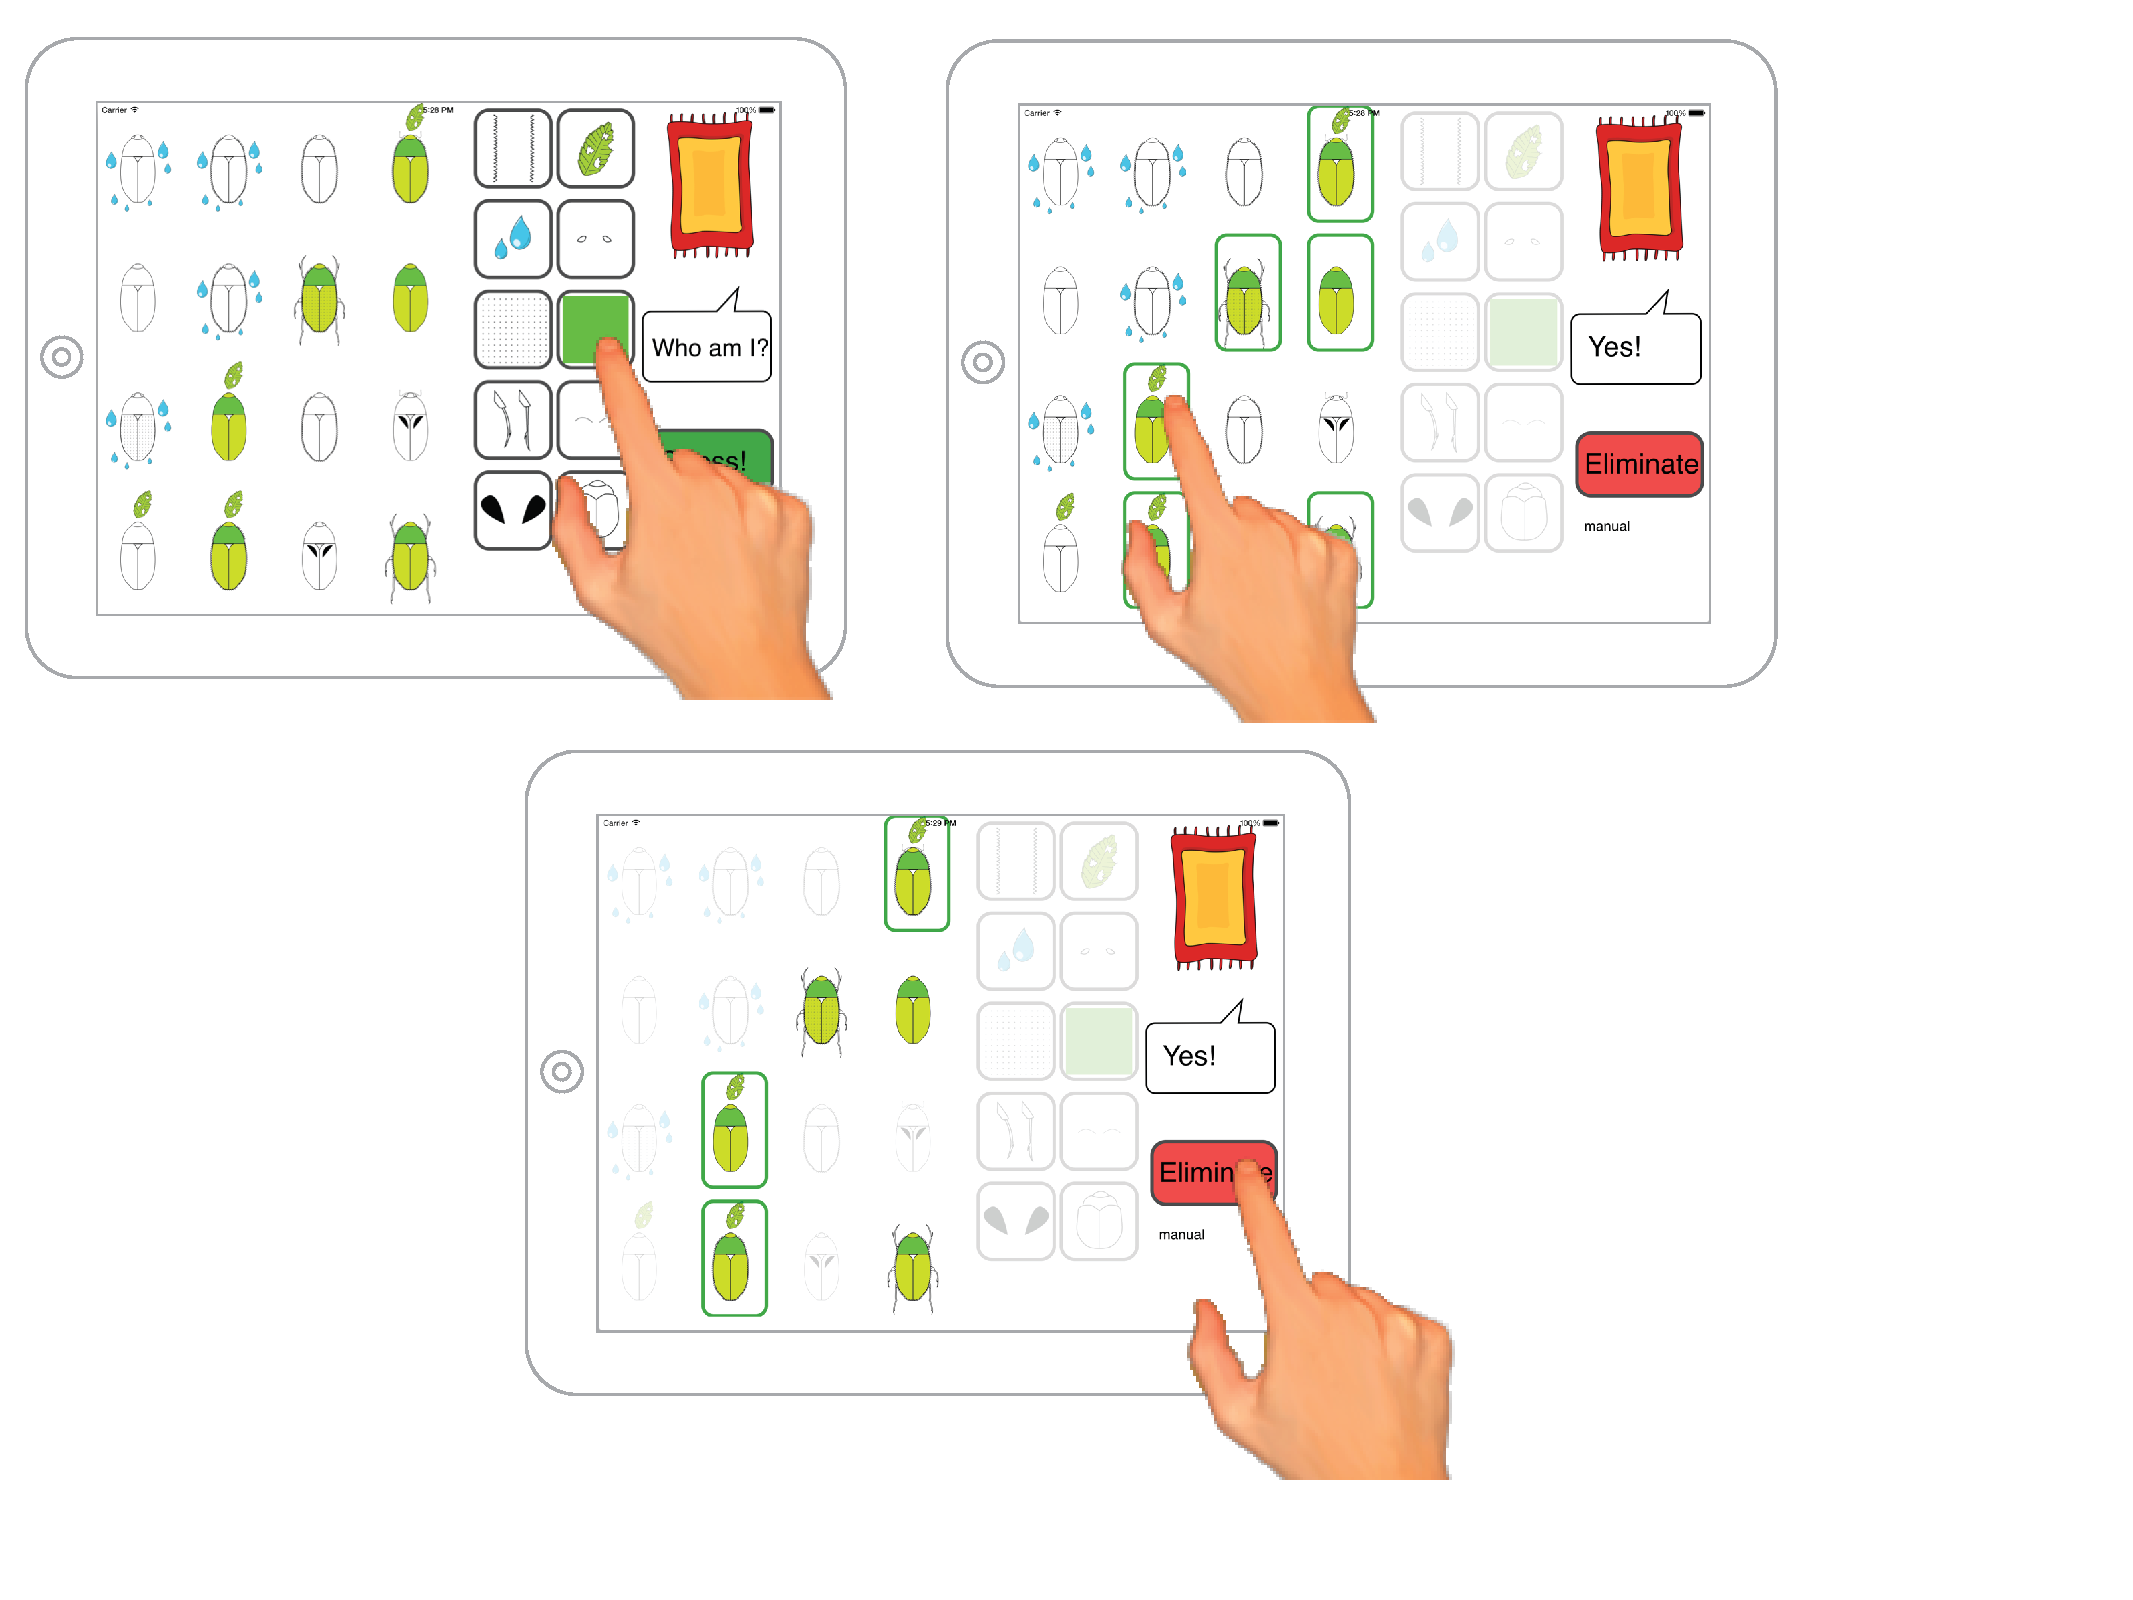
\includegraphics[width=0.7\textwidth]{figures/task_overview}
  \caption{Task overview: in the upper left, a feature button is used, asking if the insect 
hidden under the rug is green. Given feedback (``Yes!''), participants in the manual 
update condition select the insects that are consistent with this new information (upper 
right), whereas in the automatic condition the consistent insects are selected by the 
game. Players in both conditions press the red button to return to the button phase, 
and again either choose a feature button or query a single insect.}
  \label{fig:task-overview}
\end{figure} 


\subsection{Results}

\subsubsection{Overall}

% - mention that there was no effect of round!
We analyzed only the first 10 rounds of each game (only 8 children played more than 
10 rounds, including one who played 51 rounds). This covers 722 rounds from 121 
children (61 in the automatic condition and 60 in manual). The mean number of total queries (feature and exemplar) taken to complete a round was 6.5 in the automatic-update condition, and 7.6 in the manual-update condition. Although the median queries to complete a round in each condition was 6, the distributions of total queries per round for each condition were significantly different from each other (Kolmogorov-Smirnov test, $D = 0.13$, $p<.01$). 
For comparison, we simulated 700 rounds of the game with an agent that clicked randomly in the task, 
choosing uniformly at random on the first click from 16 exemplars and 10 feature buttons, and continuing with whatever stimuli (and feature queries) remain after each click, while making no update errors. This random agent took on average 8.9 queries (median: 9) to complete a round---more queries than participants in either condition.
This suggests at least some structure in children's active inquiry behavior.


\subsubsection{Qualitative Querying Behavior}

Participants' mean number of queries per round were subjected to an ANOVA with update condition 
(automatic vs. manual) and age group (5-7 vs. 8-10) as between-subjects factors and query type as 
a within-subject factor. This analysis indicated significant main effects of condition (F(1,229) = 4.60, $p<.05$) 
and age group (F(1,229) = 12.20, $p<.001$), and no significant main effect of query type 
(F(1,229) = 0.10, $p=.75$). Overall, older children required fewer queries of either type to complete a 
round ($M_{5-7} = 4.2$, $M_{8-10} = 3.3$), also evidenced by a significant negative correlation between participants' mean queries to complete a round and age ($t(119) = 3.24$, $p=.001$, $r=-.28$). There were significant interactions of condition 
and query type (F(1,229) = 22.18, $p<.001$), and age group and query type (F(1,229) = 12.25, 
$p<.001$), detailed below. No other interactions were significant (all F-values $<1$).  
In comparison to the manual condition, 
there were fewer exemplar queries in the automatic condition ($M_{man} = 5.0$, 
$M_{auto} = 3.2$, $t(103.5)=4.1$, $p<.001$), while there were more feature queries 
in the automatic condition ($M_{auto} = 3.8$) ($M_{man} = 3.3$, $t(102.9)=2.1$, 
$p<.05$).
These query rates are all lower than the simulated random rounds' mean number of feature queries (6.5) and exemplar queries (5.3), but above the optimal.\footnote{Note that although there are at first more exemplars (16) than feature buttons (10), after the first click or two there will likely be few 
exemplars remaining to click, which is why the expected number of exemplar 
queries is lower than the expected number of feature queries in the simulation.} 

Figure~\ref{fig:clicks-per-agecond} shows the average number of query types used per 
round for participants by age group. Both age groups in the manual-update condition used 
more exemplar queries than feature queries, and older participants in both conditions use fewer exemplar queries than younger participants ($M_{5-7}=4.8$, $M_{8-10}=3.0$, $t(119.0)=4.00$, $p<.001$). Older participants used a greater proportion of feature queries than younger participants in both the automatic ($M_{5-7}=.50$ vs. $M_{8-10}=.66$, $t(57.2)=3.12$, $p<.01$) 
and manual conditions ($M_{5-7}=.39$ vs. $M_{8-10}=.50$, $t(50.3)=2.30$, $p<.05$). Thus, both 
conditions replicate the \citeA{Mosher:1966} finding that older children use a greater proportion of 
constraint-seeking questions. 

\begin{figure}[h]
  \centering
  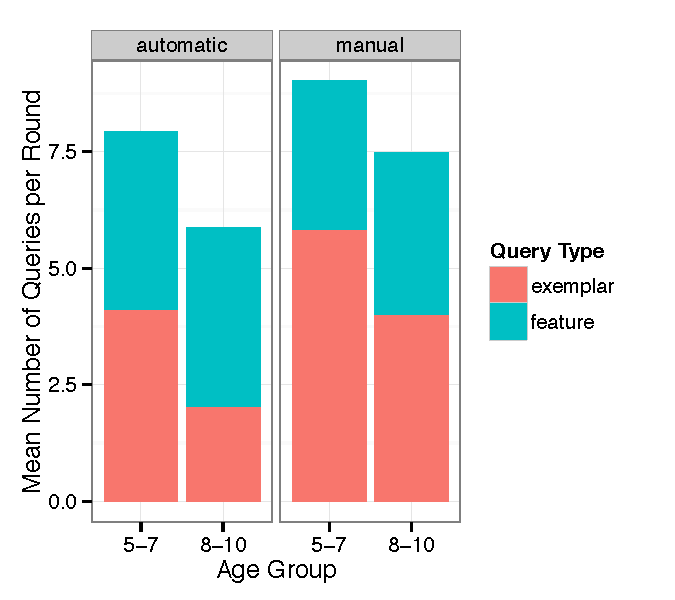
\includegraphics[width=0.55\textwidth]{figures/clicks_by_ageGroup_condition_query_type}
  \caption{Mean number of queries of each type per round by age and condition. Older children use fewer exemplar queries than younger children. Manual-update participants used more exemplar queries and fewer feature queries than automatic-update participants.}
  \label{fig:clicks-per-agecond}
\end{figure} 

% Todd: insect/bug issue the feature query/constraint seeking thing is a terminology confusion.  
% personally i like feature/exemplar but in order to connect with the developmental literature maybe we should use the other?
The finding of more feature queries in the automatic condition and more exemplar queries in the manual condition raises a number of questions about when and why participants are choosing particular queries in each condition. We next investigate response times to reveal how much thought participants are putting into making each type of query.
%Are participants reluctant to use feature queries in the manual condition because of the difficulty of updating the hypothesis space? When manual-update participants do use a feature query, do they think more carefully about which feature they choose? 

% \begin{figure}[!h]
% \centering
%  \includegraphics[width=0.5\textwidth]{figures/query_type_prop_by_round}
%  \caption{Proportion of feature vs. item queries by round.}
%  \label{fig:query-prop-round}
% \end{figure} 
 % \vspace{.05cm}
  
 
\subsubsection{Response Times}

Participants' median RT for each button type (feature and exemplar) was computed and these data were subjected to an ANOVA with condition (automatic, manual) and age group (5-7, 8-10) as 
between-subjects factors and button type as a within-subject factor. There
were significant main effects of button type (F(1,229) = 42.52, $p<.
001$) and condition (F(1,229) = 4.14, $p<.05$), but not a significant main effect of age group (F(1,229) = 0.73). On average, participants took longer to make queries in the manual 
condition (4800 ms) than in the automatic condition (4000 ms). Overall, participants took much 
longer to make feature queries (7,470 ms) than to press an exemplar button (2,680 ms), 
perhaps indicating more thought before making more complex queries. There was also a significant 
interaction effect of query type and condition (F(1,234) = 11.85, $p<.001$). Figure~\ref{fig:basic-rt} shows 
the mean of subjects' median RTs for each query type, split by condition. Feature queries were 
slower in the manual-update condition (7900 ms vs. 5430 ms in automatic), which could indicate 
1) more careful thought given to features in this condition, and/or 2) general hesitance to use feature 
queries, perhaps because it is time-consuming (even difficult) to manually update hypotheses. 
Exemplar queries were faster in the manual-update condition (1850 ms vs. automatic: 2570),
which could be greater readiness to use the simpler strategy. Other interactions were not significant (all F-values $<1$).

\begin{figure}[h]
  \centering
  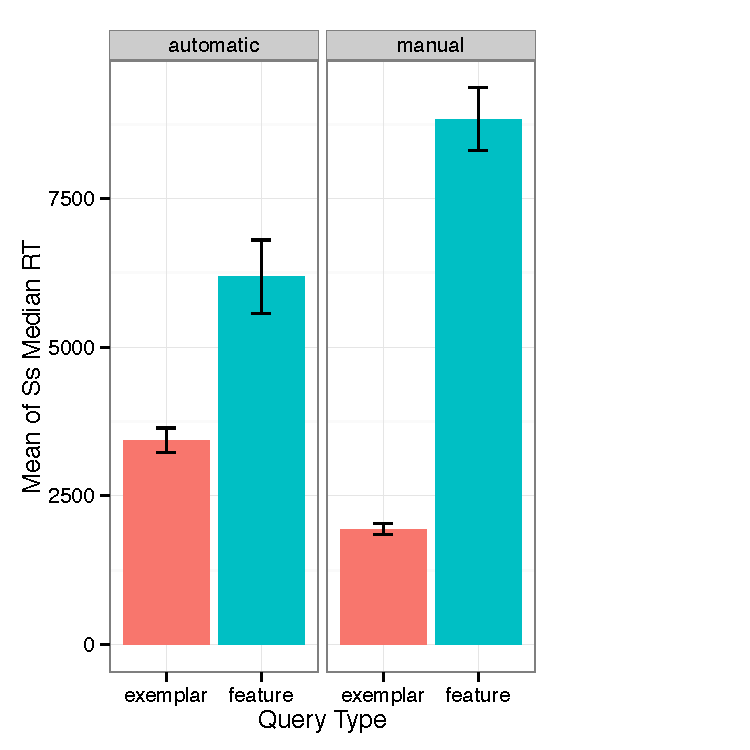
\includegraphics[width=0.55\textwidth]{figures/RT_by_condition_query_type}
  \caption{Mean of participants' median RT for each condition and query type. 
Exemplar queries were faster than feature queries, which represent a more complex 
strategy and thus likely required more thought. Feature queries were particularly slower in the 
manual-update condition. Error bars show +/-1SE.}
  \label{fig:basic-rt}
\end{figure} 

 In summary, it is clear that the manual-update condition results in fewer feature 
queries and more reliance on exemplar queries. 
Manual-update participants may be reluctant to use feature queries for at least two reasons: 1) it demands more time and cognitive effort to manually update the hypothesis space after a feature query than 
in the automatic-update condition, and 2) the manual update process is error-prone, 
and any mistakes may in turn lead to more exemplar queries in order to recover.\footnote{If the correct answer is mistakenly eliminated, exemplar queries are needed to find it and finish the round. These additional exemplar queries were excluded from analysis.} 
Therefore we proceed to investigate errors in manual updating.

\subsubsection{Manual Update Mistakes}

% make it clear the queries beyond normal round length are removed from analysis
The manual-update condition allows participants to commit two types of error during 
hypothesis updating: a miss is defined as a failure to eliminate a insect, and a false 
alarm is a failure to keep a hypothesis that was consistent with the query. Note that 
a miss is an error of commission--i.e., the insect had to be tapped to be kept--whereas 
a false alarm is an error of omission (i.e., failing to tap a insect), and thus we expect 
more of the latter. Comparing the manual-update subjects' mean number of errors of 
each type per round, indeed there were more false alarms ($M=6.9$, sd = 1.9) than 
misses ($M=1.8$, sd = 1.3; paired $t(58) = 19.8$, $p<.001$). A MANCOVA to 
determine if error rates were related to age did not find a significant effect for either 
misses (F(1,56) = 0.77, $p>.05$) or false alarms (F(1,56) = 0.23, $p>.05$).  Consistent
with our hypothesis that manual updating increases cognitive load and reduces
resource of information seeking behavior, fewer 
feature queries and more exemplar queries were made in the manual condition. 
However, RT analyses also indicated that 
feature queries took longer under manual updating.  One possibility is that
feature queries were more carefully considered in this condition than under 
the ease of automatic updating.  To evaluate this idea, we conducted a model-based
analysis children's feature queries which provides a context-sensitive measure of query
informativeness.
%
%Although the qualitative analyses have thus far revealed interesting effects that build on the previous literature, as the game unfolds the utility of different query types (and specific queries) changes, and can be best quantified using a more sophisticated model-based approach to understanding the quality of children's question asking.

\subsubsection{Expected Information Gain}

Each successive query reduces the size of the remaining hypothesis space to some degree: 
on the first move, querying the appropriate feature (F1) can cut the space in half. 
When two 
hypotheses remain, even an exemplar query will cut the space in half. 
As a result, the distinction between constraint-seeking and hypothesis scanning
queries in not absolute (either could be better in different circumstances).
As describe in the Introduction, one way to analyze the contextual sensitivity 
of participants' queries is to calculate the Expected 
Information Gain (EIG) of the query they made. 

We first introduce key terms used to 
define EIG. Entropy measures uncertainty about the outcome of a random variable 
$X$ and is denoted $H(X)$. Entropy is 0 when there is only one possible outcome, and maximal when all 
possible outcomes are equiprobable (i.e., a uniform distribution).

\begin{equation}
  H(X) = -\sum_{x} p(x) \cdot log(p(x))
\end{equation}

Mutual information gain, $I(X;Y)$, measures the change in entropy as we receive a new piece 
of information $Y$, i.e., how much does our uncertainty about X change given that 
we know Y?

\begin{equation}
  I(X;Y) = H(X) - H(X|Y)
\end{equation}

The Expected Information Gain (EIG) of a query $Q$ is the weighted average of the 
information possible from each possible answer to the query, weighted by the 
current probability of receiving that answer. This will be 0 (or near-0) for queries that 
can be expected to eliminate none or just one or two hypotheses in a large space, 
and more positive for queries that are likely to eliminate a larger number of 
hypotheses. In this task, EIG is maximal (1) for a feature query that will eliminate 
half the remaining hypotheses. Such a query is always available at the beginning of 
any round, and due to the partially-nested feature structure used, maximal EIG 
queries are often available at other stages of the round.

\begin{equation}
  EIG(Q) = -\sum_{Y} p(Y|Q) I(X;Y)
\end{equation}

% moved discussion of EIG use to study children's decisions to intro
We analyze the EIG for each participants' feature queries separately, as well as in aggregate with the exemplar queries
\footnote{Exemplar query EIGs alone are less interesting, as they are a simple function of how many hypotheses 
remain. Participants' choice of feature query, on the other hand, indicates how 
sensitive they are to the relevance of each feature--and to the context of their 
current situation. However, as the space shrinks, it is interesting to see whether participants' persist in making (now less informative) feature queries, or switch to (increasingly informative) exemplar queries.} 
Participants' mean feature query EIG was 
subjected to an ANOVA with condition and age group (5-7 vs. 8-10) as between-subjects factors. 
This ANOVA indicated significant main effects of condition (F(1,115) = 55.0, $p<.001$) 
and age group (F(1,115) = 12.42, $p<.001$), with no significant interaction effect (F(1,115) = 0.2, $p>.05$).\footnote{The same significant effects and similar mean EIG values were obtained when analyzing only the first two feature queries per round, when manual- and automatic-update participants were on more equal footing (i.e., before further manual errors--which could raise or lower the EIG of the remaining feature queries).}
The same ANOVA applied to participants' mean EIG of all queries indicated a marginally-significant main effect of condition (F(1,116) = 3.29, $p=.07$) and a significant main effect of age group (F(1,116) = 25.70, $p<.001$).
Figure~\ref{fig:EIG_by_age} shows mean EIG per feature query (left) and for all queries (right) by age group and condition, along with a baseline simulation showing the mean EIG of all the feature queries (i.e., as if each subject had chosen randomly from the feature queries). Note that although randomly-chosen features for the manual-update subjects have a higher EIG than for automatic-update subjects (driven in part by update errors quickly reducing the hypothesis space), the simulated random EIGs are far below the corresponding human data.
Mean EIG of feature queries for each subject was marginally significantly correlated with 
age ($t(116)=1.77$, $p=.08$, $r=.16$), showing that older children tended to use more relevant feature queries. 
The feature queries made by participants in the 
automatic condition had significantly lower EIG than those made in the manual 
condition ($M_{auto} = .60$, $M_{man} = .74$, $t(116) = 5.49$,  $p<.001$). Thus, 
although manual-update participants used fewer feature queries overall, and tended 
to make mistakes during hypothesis updating, they
queried features with higher expected information gain than automatic-update 
participants. Along with the reaction time results described above, this suggests that these children 
thought more before making their choices and in fact performed better.  Indeed, there was a weak but significant 
correlation of participants' mean feature query RT and EIG ($r=.20$, $t(116)=2.17$, $p<.05$), verifying that longer 
RTs are associated with more informative feature queries.
% information gain conditioned on what they know? (duplicate feature clicks?

\begin{figure}[t]
  \begin{subfigure}{.42\textwidth}
  \centering
  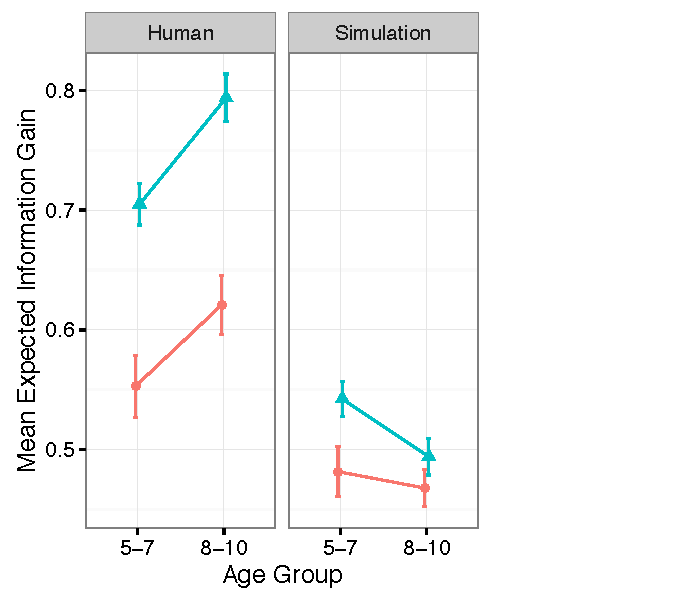
\includegraphics[width=.9\linewidth]{figures/EIG_by_ageGroup_n_condition_with_random_sims}
  \caption{Mean EIG for feature queries.}
  \label{fig:sfig1}
\end{subfigure}%
\begin{subfigure}{.58\textwidth}
  \centering
  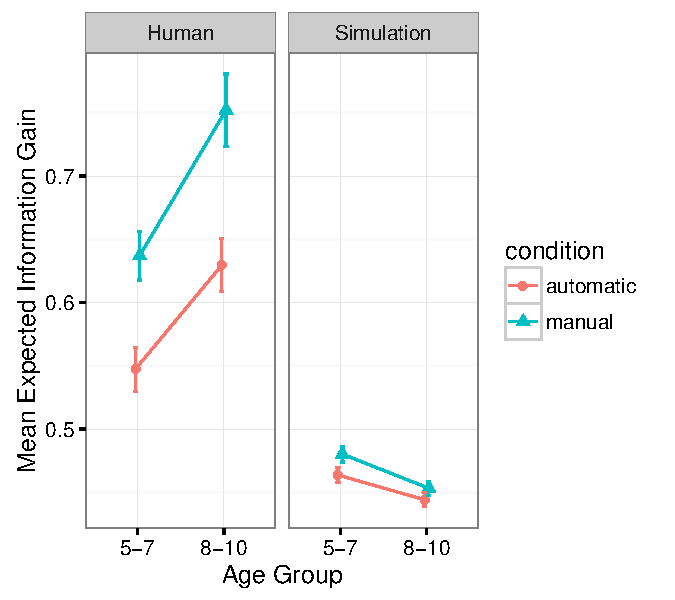
\includegraphics[width=.9\linewidth]{figures/EIGall_by_ageGroup_n_condition_with_random_sims}
  \caption{Mean EIG for all queries.}
  \label{fig:sfig2}
\end{subfigure}
 \caption{Mean expected information gain for feature queries by age group and condition, 
with a simulation making random feature queries--in the same situations as subjects (not the earlier random agents)--for comparison. Manual-update subjects had higher EIG than automatic-update subjects, and both were better than random--but suboptimal (1). Older children had higher EIG than younger children. Bars show +/-1SE.}
\label{fig:EIG_by_age}
 % 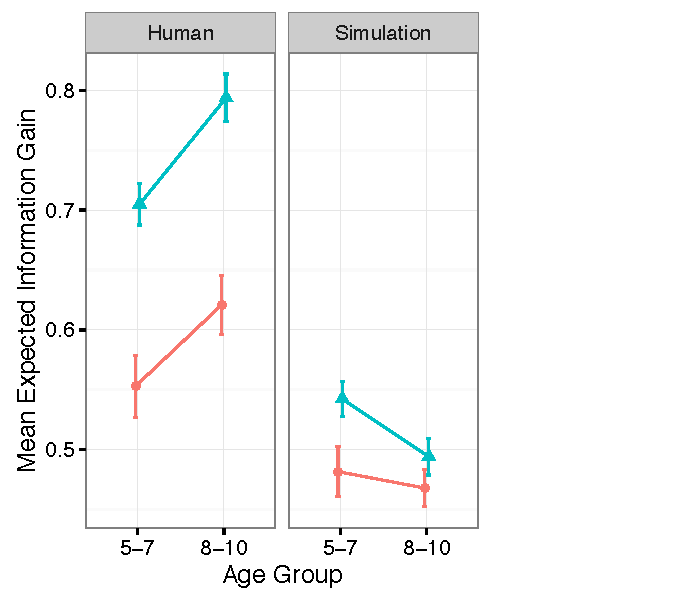
\includegraphics[width=0.55\textwidth]{figures/EIG_by_ageGroup_n_condition_with_random_sims}
 % \caption{}
 % \label{fig:EIG_by_age}
\end{figure} 

\subsubsection{Click-by-click behavior}
%Individual strategies: mostly exemplar vs. feature queries? 

Figure~\ref{fig:query-prop-click} shows the mean proportion of feature vs. exemplar queries by click index within a round for each update condition split by age group, contrasted with simulated agents choosing any available buttons uniformly at random throughout the game. Older children show a much higher proportion of feature queries in the first three clicks of the automatic condition, and the first two of the manual condition. In both update conditions, the first three clicks are more likely to be feature than exemplar queries, and automatic-update subjects often make a fourth feature query before likely moving to exemplar queries. 
Both human conditions are quite different than the simulated random agent. 
Rather, the response profile of human participants looks generally like the optimal sequence: 3 feature queries and then one (sometimes two) exemplar queries. However, as was shown earlier, participants rarely chose the most informative feature to query at any given time, and manual participants made a number of updating errors. Where does the higher EIG for manual-update feature queries come from? Are they choosing the best feature query from the start, or are they simply better at testing more contextually-relevant features later in the round?

Figure~\ref{fig:EIG_by_click} shows the mean EIG of feature queries by feature query index (left), and for all queries (right), with a simulation based on the participants' data for comparison: although following the same sequence of situations as participants, this simulation shows the EIG if a query (just feature at left, or feature and exemplar at right) had been chosen at random in each instance. 
Figure~\ref{fig:EIG_by_click} reveals that people in the two update conditions had similarly informative first queries--especially for the 5-7 year-olds, who were not much better than random, but that manual subjects' subsequent few feature queries were more informative than automatic subjects' or the random choices. That is to say, manual-update participants chose feature queries that were more contextually appropriate for the particular set of remaining hypotheses, in contrast to automatic-update participants who--despite finding an informative feature for the first query--paid less attention to the unfolding situation. In fact, after the initial high-quality query, the younger automatic-update participants chose queries with nearly the same EIG as the random simulation, implying that they more or less ignored the features of the remaining hypotheses. For older automatic-update participants, feature query EIG was better than random after the first query, although it remained below manual-update EIG across feature queries.
%Feature queries are made at a rate that is correlated with the number of exemplars 
%they are relevant to ($r=.79$, $t(8)=3.6$, $p<.01$). 

\begin{figure}[t] % [!h]
  \centering
  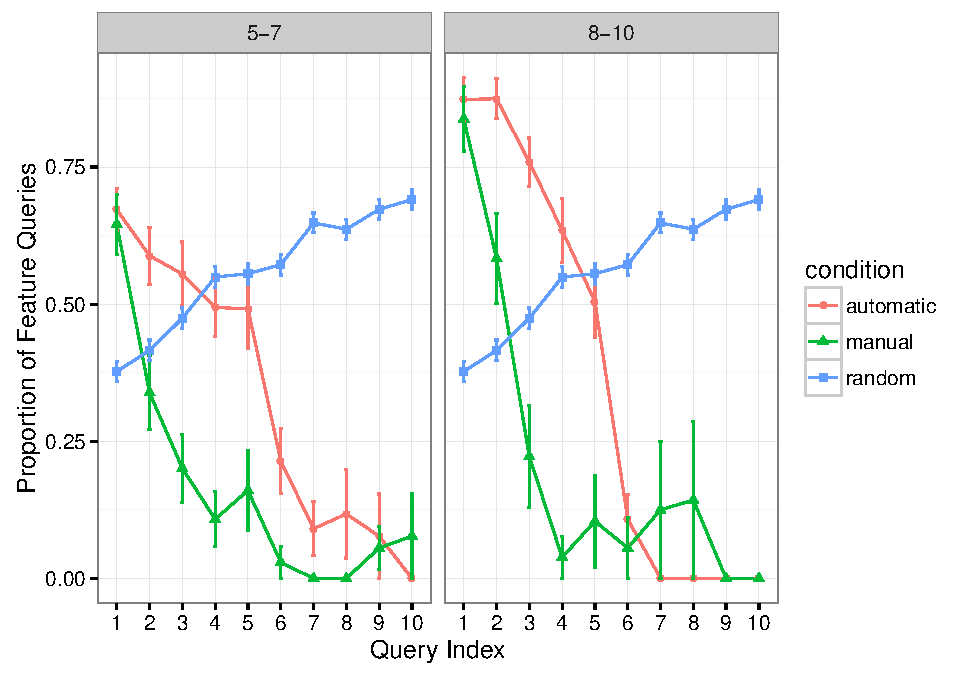
\includegraphics[width=0.75\textwidth]{figures/proportion_feat_queries_by_click} % 
  \vspace{-.1cm}
  \caption{Proportion of feature vs. exemplar queries by click for each update condition, with a randomly-clicking agent for comparison. People in both conditions are more likely to make feature queries rather than 
exemplar queries in the first three clicks of a round, but manual-update participants 
move more quickly to exemplar queries, and are overall more likely to make 
exemplar queries. Older children make a higher proportion of feature queries in the first few clicks of both conditions.}
  \label{fig:query-prop-click}
  \vspace{-.1cm}
\end{figure} 




 \begin{figure}[t] %[!h]
 %\centering
  \begin{subfigure}{.57\textwidth}
  \centering
  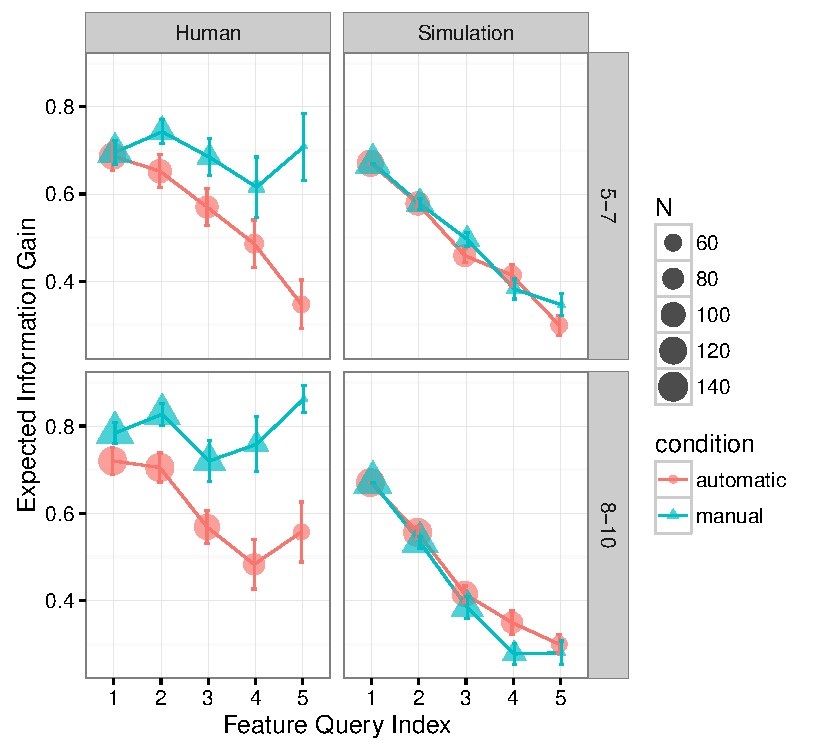
\includegraphics[width=.98\linewidth]{figures/info_gain_by_click_n_age_w_sims}
  \caption{Mean EIG by feature query.}
  \label{fig:sfig1}
\end{subfigure}%
\begin{subfigure}{.43\textwidth}
  \centering
  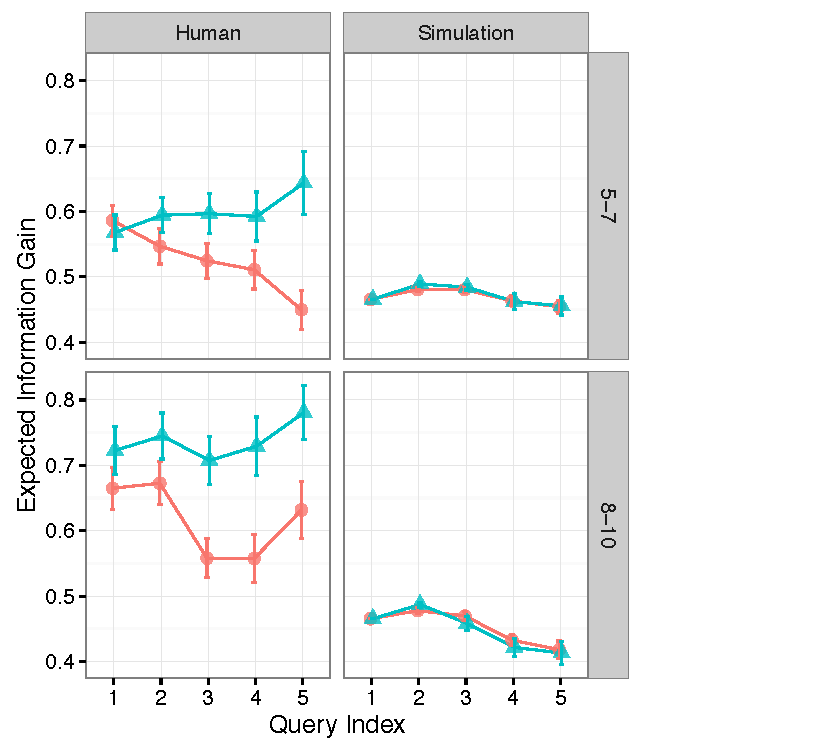
\includegraphics[width=.98\linewidth]{figures/all_info_gain_by_click_n_age_w_sims}
  \caption{Mean EIG by all queries.}
  \label{fig:sfig2}
\end{subfigure}
  %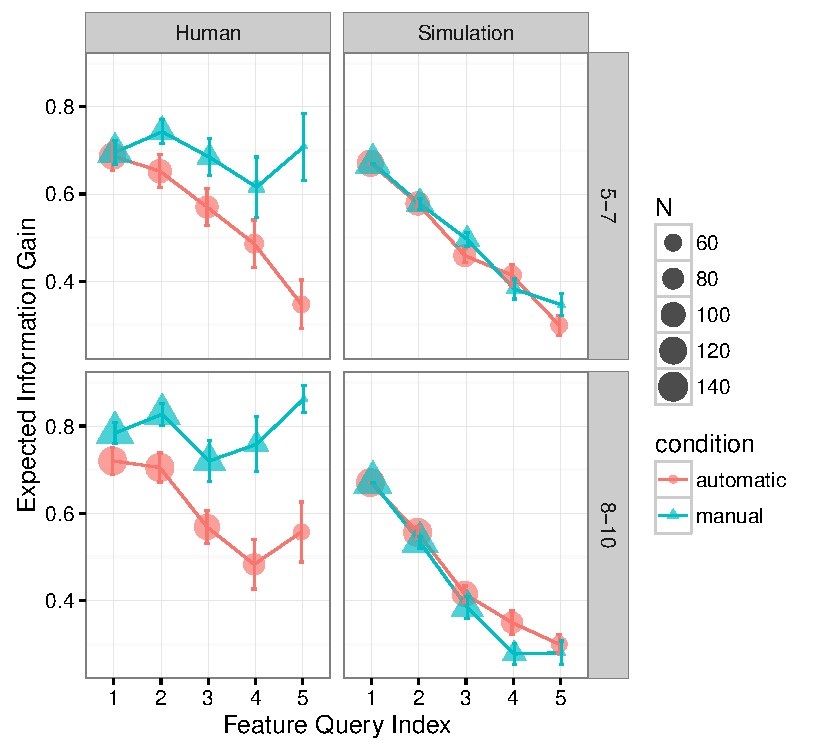
\includegraphics[width=0.55\textwidth]{figures/info_gain_by_click_n_age_w_sims} % info_gain_by_click_w_sim_w_N
  \caption{Subjects' mean expected information gain (EIG) of feature queries (left) and all queries (right) by click index by condition. At left, although the first feature query--made when the full hypothesis space is possible--had nearly the same mean EIG in both conditions, the next few feature queries in the manual-update condition had higher mean EIG than the automatic condition. This suggests that manual-update subjects paid more attention to the remaining hypotheses after the first query, and made subsequent feature queries that were sensitive to the current context. Making four or more feature queries in a given round was quite rare, as most participants mostly switched to exemplar queries after the second or third feature query. EIG for all queries (right) show a similar pattern (and a stronger advantage over the simulation), meaning that manual participants are better at switching to exemplar queries at the right time, whereas automatic participants may be persisting in querying (now uninformative) features. Bars show +/-1SE.}
  \label{fig:EIG_by_click}
 \end{figure} 


% \begin{figure}[t]  %[!h]
 %\centering
 % 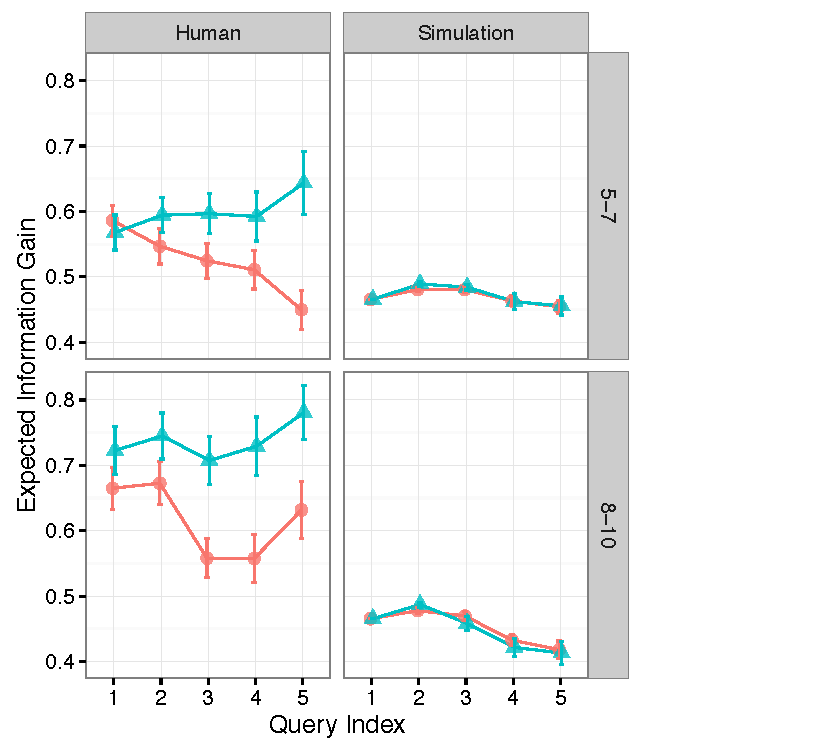
\includegraphics[width=0.55\textwidth]{figures/all_info_gain_by_click_n_age_w_sims} % info_gain_by_click_w_sim_w_N
 % \caption{Subjects' mean expected information gain (EIG) of all queries by click index by condition, with symbol size indicating frequency of occurrence. Bars show +/-1SE.}
%  \label{fig:EIGall_by_click}
% \end{figure} 

\section{General Discussion}

The present study asked children 5-10 years of age to learn feature distributions in an unfamiliar hypothesis space, and examined both their qualitative questioning strategies, and how efficiently they were able to search that space. Previous studies have examined question asking in somewhat familiar hypothesis spaces \cite{Herwig:1982,Mosher:1966,Nelson:2014,Ruggeri:2014,Ruggeri:2015}, but no study we are aware of has considered the step of updating the hypothesis space when new evidence is received--let alone in a novel hypothesis space. In many previous developmental studies, experimenters help children update the remaining hypothesis, quite reasonably: this step is potentially quite challenging, especially for younger children.  Importantly, we manipulated the support children were  given while updating the hypothesis space: after a feature query, participants in the 
automatic update condition were shown which insects were eliminated at the press of 
a button, whereas manual update participants were required to select the insects that 
were consistent with the feedback. 

In line with previous research \cite{Mosher:1966,Ruggeri:2014}, the present study found older children (ages 8-10) asked a higher proportion of constraint-seeking questions than younger children (ages 5-7), who relied more on hypothesis-scanning (i.e., exemplar queries), in both conditions. These qualitative analyses also found that children use more constraint-seeking questions (i.e., feature queries) in the automatic-update condition. On the surface then, these children were using a more efficient strategy than the manual-update children. % suggesting...
From this qualitative analysis alone, then, it is tempting to conclude that automatic updating leads to a better querying strategy than manual updating.

However, in terms of expected information gain, a context-sensitive measure of how well a chosen feature bisects the remaining hypothesis space, it turned out that children in the 
automatic-update condition made less informative feature queries. We 
suggest that the greater mental effort required by manual updating actually lead 
to more careful consideration of which feature query to use, and ultimately a better choice. Indeed, response times for feature queries were slower under manual updating, indicating that greater thought went into making those choices, corroborated by the fact that slower feature query RTs were correlated with more informative queries. Within-round analysis found that automatic-update participants were likely to make feature queries for the first few clicks, while manual-updaters switched often switched to exemplar queries after one (5-7 year-olds) or two feature queries (8-10 year-olds). In terms of quality, feature queries in both update conditions were similar for the first query in a round--and better than the simulation. However, manual-update subjects made more contextually-sensitive feature queries after the first query, whereas automatic-update participants looked much like they were choosing random feature queries, without regard for the current hypothesis space's features. In both conditions, older children made more informative feature queries, but even 5-7 year-olds asked far more informative questions than a random simulation, showing some efficiency in navigating an unfamiliar domain even after only a few minutes of experience. 

In summary, this study provides evidence that hypothesis updating is a difficult, error-prone step in the active inquiry process. Moreover, children of all ages tested here (5- to 10-years-old) are sensitive to the difficulty of this step: when aided in hypothesis updating, asked more constraint-seeking questions than when they had to manually update the space. However, we also uncovered evidence of a desirable difficulty in this step: manual updating resulted in more informative, contextually-sensitive constraint-seeking questions than the supported update process. Surprisingly, even younger children (5- to 7-year-olds) in the manual-update condition made feature queries with higher expected information gain than their peers in the automatic-update condition. Future work will aim to reduce errors in manual hypothesis updating via intervention, and will aim to uncover other bottlenecks--or desirable difficulties--in active inquiry. 

Finally, it is worth noting that this partially self-guided iPad study was conducted in the relaxed learning environment of the American Museum of Natural History's Discovery Room. 
Children's developing abilities to engage in the basic steps of scientific 
 thinking are on full display in such informal science learning environments, such as at 
science and children's museums. Indeed, a central goal of these environments is to 
provide children with hands-on opportunities to learn from their own explorations, to 
enable them to gain active experience with the steps of scientific investigation, to 
discover new knowledge, and to develop enthusiasm for and interest in science 
\cite{Bell:2009,Fenichel:2010}. As a result, informal science 
environments may provide an excellent domain in which to investigate the development of understanding. This study demonstrates that such environs can be suitable and fruitful venues for knowledge discovery not only for children, but for scientists, too.

\section{Acknowledgments}

This work was supported by the John Templeton Foundation 
``Varieties of Understanding" grant to TMG and MR. 
We are grateful to Kathryn Yee, Aja Blanco, Christina Chu, and Talena Smith for data collection, and to Daniel Zeiger and the staff of the Discovery Room at the American Museum of Natural History for their support of this project.

\bibliographystyle{apacite}

%\setlength{\bibleftmargin}{.125in}
%\setlength{\bibindent}{-\bibleftmargin}

\bibliography{sensemaking_refs}

\end{document}
